%%%%%%%%%%%%%%%%%%%%%%%%%%%%%%%%%%%%%%%%%%%%%%%%%%%%%%%%%%%%%%%%%%%%%%%%%%%%
% AGUJournalTemplate.tex: this template file is for articles formatted with LaTeX
%
% This file includes commands and instructions
% given in the order necessary to produce a final output that will
% satisfy AGU requirements, including customized APA reference formatting.
%
% You may copy this file and give it your
% article name, and enter your text.
%
%
% Step 1: Set the \documentclass
%
%

%% To submit your paper:
\documentclass[draft]{agujournal2019}
\usepackage{url} %this package should fix any errors with URLs in refs.
\usepackage{lineno}
\usepackage[inline]{trackchanges} %for better track changes. finalnew option will compile document with changes incorporated.
\usepackage{soul}
\usepackage{amsmath}
\linenumbers
%%%%%%%
% As of 2018 we recommend use of the TrackChanges package to mark revisions.
% The trackchanges package adds five new LaTeX commands:
%
%  \note[editor]{The note}
%  \annote[editor]{Text to annotate}{The note}
%  \add[editor]{Text to add}
%  \remove[editor]{Text to remove}
%  \change[editor]{Text to remove}{Text to add}
%
% complete documentation is here: http://trackchanges.sourceforge.net/
%%%%%%%

\draftfalse

%% Enter journal name below.
%% Choose from this list of Journals:
%
% JGR: Atmospheres
% JGR: Biogeosciences
% JGR: Earth Surface
% JGR: Oceans
% JGR: Planets
% JGR: Solid Earth
% JGR: Space Physics
% Global Biogeochemical Cycles
% Geophysical Research Letters
% Paleoceanography and Paleoclimatology
% Radio Science
% Reviews of Geophysics
% Tectonics
% Space Weather
% Water Resources Research
% Geochemistry, Geophysics, Geosystems
% Journal of Advances in Modeling Earth Systems (JAMES)
% Earth's Future
% Earth and Space Science
% Geohealth
%
% ie, \journalname{Water Resources Research}

\journalname{Journal of Advances in Modeling Earth Systems (JAMES)}


\begin{document}

%% ------------------------------------------------------------------------ %%
%  Title
%
% (A title should be specific, informative, and brief. Use
% abbreviations only if they are defined in the abstract. Titles that
% start with general keywords then specific terms are optimized in
% searches)
%
%% ------------------------------------------------------------------------ %%

% Example: \title{This is a test title}

\title{Design and implementation of a data-driven parameterization for mesoscale thickness fluxes}

%% ------------------------------------------------------------------------ %%
%
%  AUTHORS AND AFFILIATIONS
%
%% ------------------------------------------------------------------------ %%

% Authors are individuals who have significantly contributed to the
% research and preparation of the article. Group authors are allowed, if
% each author in the group is separately identified in an appendix.)

% List authors by first name or initial followed by last name and
% separated by commas. Use \affil{} to number affiliations, and
% \thanks{} for author notes.
% Additional author notes should be indicated with \thanks{} (for
% example, for current addresses).

% Example: \authors{A. B. Author\affil{1}\thanks{Current address, Antartica}, B. C. Author\affil{2,3}, and D. E.
% Author\affil{3,4}\thanks{Also funded by Monsanto.}}

\authors{Dhruv Balwada\affil{1}, 
Pavel Perezhogin\affil{2}, 
%Ryan Abernathey\affil{4}, 
Alistair Adcroft\affil{4}, 
and Laure Zanna\affil{2,3}}  


% \affiliation{1}{First Affiliation}
% \affiliation{2}{Second Affiliation}
% \affiliation{3}{Third Affiliation}
% \affiliation{4}{Fourth Affiliation}

\affiliation{1}{Lamont-Doherty Earth Observatory, Columbia University, Palisades, NY, USA}
\affiliation{2}{Courant Institute of Mathematical Science, New York University, New York, NY, USA}
\affiliation{3}{Center for Data Science, New York University, New York, NY, USA}
\affiliation{4}{Princeton University, Princeton, NJ, USA}


%(repeat as many times as is necessary)

%% Corresponding Author:
% Corresponding author mailing address and e-mail address:

% (include name and email addresses of the corresponding author.  More
% than one corresponding author is allowed in this LaTeX file and for
% publication; but only one corresponding author is allowed in our
% editorial system.)

% Example: \correspondingauthor{First and Last Name}{email@address.edu}

\correspondingauthor{Dhruv Balwada}{dbalwada@ldeo.columbia.edu}

%% Keypoints, final entry on title page.

%  List up to three key points (at least one is required)
%  Key Points summarize the main points and conclusions of the article
%  Each must be 140 characters or fewer with no special characters or punctuation and must be complete sentences

% Example:
% \begin{keypoints}
% \item	List up to three key points (at least one is required)
% \item	Key Points summarize the main points and conclusions of the article
% \item	Each must be 140 characters or fewer with no special characters or punctuation and must be complete sentences
% \end{keypoints}

\begin{keypoints}
\item A data-driven mesoscale thickness flux parameterization was designed and implemented in MOM6 as an alternative to the Gent-McWilliams scheme 
\item The parameterization is stable and skillful across a range of resolutions including the eddy-permitting gray zone
\item The parameterization is able to reduce potential energy without overly dissipating the resolved eddy energy
\end{keypoints}

%% ------------------------------------------------------------------------ %%
%
%  ABSTRACT and PLAIN LANGUAGE SUMMARY
%
% A good Abstract will begin with a short description of the problem
% being addressed, briefly describe the new data or analyses, then
% briefly states the main conclusion(s) and how they are supported and
% uncertainties.

% The Plain Language Summary should be written for a broad audience,
% including journalists and the science-interested public, that will not have 
% a background in your field.
%
% A Plain Language Summary is required in GRL, JGR: Planets, JGR: Biogeosciences,
% JGR: Oceans, G-Cubed, Reviews of Geophysics, and JAMES.
% see http://sharingscience.agu.org/creating-plain-language-summary/)
%
%% ------------------------------------------------------------------------ %%

%% \begin{abstract} starts the second page

\begin{abstract}
% The question is 
Mesoscale eddies are a major sink of available potential energy (APE) in the ocean. When these eddies are not resolved or only partially resolved in a model, this effect needs to be parameterized to simulate a realistic large-scale state. Traditionally, the Gent-McWilliams (GM) parameterization has provided this sink of APE. However, GM parameterization, which diffuses isopycnal heights, is not accompanied by any skillful prescription for the GM diffusivity rooted in data from observations or models. Also, at eddy permitting resolutions, the GM diffusion is known to negatively impact the resolved eddies, and the only scale-aware prescription is to turn GM off in model regions where eddies are permitted.  
% Here we do 
Here we present a novel data-driven parameterization, as a substitute to the GM parameterization, that is able to extract APE without any overly negative impacts to the resolved flow. The parameterization is also flow-aware and scale-aware, and its magnitude can be adjusted with the help of an O(1) non-dimensional number.
% What we found 
Aspects like non-dimensional inputs and outputs, lateral non-locality, flow dependent coordinates and range limitations have been incorporated to improve the generalization aspects of the data-driven parameterization. Also the functional forms are learned via a small multi-layer perceptron, allowing for low computational cost and ease of implementation into numerical ocean models. 
The parameterization is found to be highly skillful in offline evaluation, particularly at scales smaller than the size of the largest eddies.
The parameterization is implemented into NOAA GFDL$'$s MOM6, and shown to be skillful in online evaluations performed in 2 layer idealized simulations of zonal channel and wind-driven gyre, at both eddy permitting and non-eddying resolutions. 
%How it matters 
\end{abstract}

\section*{Plain Language Summary}
Mesoscale (~100 km) eddies are the dominant flows in the ocean and play a key role in shaping large-scale circulation features such as wind-driven gyres and the meridional overturning circulation. Since these eddies are not fully resolved in many modern ocean models — especially those that are run for long periods or include many ensemble members — their effects must be represented through parameterizations. A commonly used approach, the Gent-McWilliams (GM) parameterization, removes available potential energy (APE) from the system but lacks a data-driven way to set its strength. Moreover, at eddy-permitting resolutions, GM can interfere with the resolved flows.

We present a new data-driven parameterization designed to better represent eddy effects in ocean models. It learns a functional form from high-resolution simulations using a compact neural network and is designed to be flow-aware, scale-aware, and computationally efficient. The parameterization is implemented in the MOM6 ocean model and shows skillful performance both offline and in idealized simulations, especially at scales smaller than the largest eddies. It extracts APE from large scale flow without degrading resolved features, offering a promising alternative to GM for a wide range of ocean modeling applications.

%% ------------------------------------------------------------------------ %%
%
%  TEXT
%
%% ------------------------------------------------------------------------ %%

%%% Suggested section heads:
\section{Introduction}
% Big problem in science 
Ocean circulation models solve equations describing the motions in the ocean on a finite-size discrete grid, and are thus unable to resolve the phenomena at scales smaller than the grid scales. However, it is often the case that these \textit{sub-grid} phenomena are more than just small-scale variability, and could have a profound impact on the characteristics of the resolved motions. To ensure fidelity of the model behavior at the resolved scales, the effects of these sub-grid phenomena need to be appropriately \textit{parameterized}. One important and often unresolved range of scales in ocean models are the mesoscales. 

%Oceanic flows are replete with mesoscale eddies (scales of $\sim50-200$km). 
Mesoscales ($\sim50-200$km) are the dominant energy-containing scales in the ocean \cite{ferrari2009ocean}, and subsequently play an important role in shaping the mean circulation and stratification \cite{gent2011gent}, and in transporting tracers \cite{abernathey2015phase}. These eddies are believed to be largely generated as a result of baroclinic instability \cite{gill1974energy, smith2007geography}, which has its fastest growth rate at scales close to the first baroclinic deformation radius (scales of $\sim10-100$km) \cite{chelton1998geographical, tulloch2011scales}. These instabilities have a tendency to grow at the expense of the available potential energy (APE), and thus their bulk effect is to flatten isopycnals in the ocean. The dominance of rotation at these scales also usually leads to a subsequent inverse energy cascade, which is why the dominant peak of energy is usually larger than the dominant scale of the instability \cite{tulloch2011scales}. 
Thus, to properly resolve these eddies and their effects the model grid spacing needs to be at least as small as the deformation radius \cite{hallberg2013using}. The inverse cascade also takes place in the vertical \cite{smith2002scales}, transferring energy to the barotropic and first couple of baroclinic modes, and the associated flows tend to have weak vertical shear and do not generate small-scale turbulence or diapycnal mixing --- mesoscale eddies are dominantly adiabatic processes in the interior of the ocean. 


% Narrower problem within
Conventionally, mesoscale eddy effects have been parameterized using the Gent-Mcwilliams (GM) parameterization \cite{gent1990isopycnal}, particularly in models that do not resolve the deformation radius. This parameterization was designed to respect two important aspects of mesoscale processes: (i) the parameterization is adiabatic, and (ii) the net effect of the parameterization is to reduce available potential energy. 
In models with depth as the vertical coordinate, this is achieved by representing the horizontal eddy fluxes in the form of a horizontally downgradient buoyancy diffusion and then setting the vertical component of the eddy flux to be upgradient, such that the net flux is along isopycnals and the resulting operator behaves like advection. 
In contrast in isopycnal models, this is achieved by diffusing the interface heights, which can also be represented as extra eddy driven advection. 
These recipes led to dramatic qualitative improvements in the ocean simulations, particularly the adiabatic aspect ensures that water masses were not eroded away in the interior by spurious diffusion. However, the associated eddy diffusivity has always been a major source of uncertainty and a very active topic of research for decades \cite<e.g.>[]{visbeck1997specification, ferreira2005estimating, eden2008towards, marshall2012framework, jansen2015parameterization}. Also, as with all conventional ocean parameterizations, this scheme was designed to represent the bulk effects of eddies and not to have any skill in representing the spatial or temporal structures of the eddy effects, which leads to detrimental effects at resolutions where eddies are partially resolved \cite{hallberg2013using, mak2023scale}.

% Evaluation of a scalar eddy transport coefficient based on geometric constraints, Bachman 2017 gives a nice concise overview of some methods to approximate the eddy diff. 

In recent years, machine learning (ML) based methods have started to show a lot of promise in improving different aspects of computational modeling, including improving parameterizations \cite{bracco2025machine, lai2024machine}. While conventional parameterizations require domain scientists to develop mathematical operators that are at best able to mimic the bulk effects of sub-grid phenomena, ML methods directly learn the functional relationship between the sub-grid effects and the large-scale fields using appropriate data. In some instances it is also possible to design the ML models to obey physical properties through modifications to the architectural design or the loss function \cite{beucler2021enforcing, zanna2020data}. These methods have led to the development of parameterizations for idealized systems \cite{ross2023benchmarking, srinivasan2023turbulence}, thermodynamic and momentum tendencies in the atmosphere \cite{brenowitz2018prognostic, yuval2021use}, boundary layers processes in the ocean \cite{sane2023parameterizing, ramadhan2020capturing, bodner2023data}, and momentum tendencies in the ocean \cite{zhang2023implementation, zanna2020data, perezhogin2024stable}. All these new parameterizations have shown improved skill over conventional parameterizations, and the potential issues raised about implementation, stability and generalization are rapidly being addressed.  
While some sub-grid effects of ocean eddies have been investigated using this approach, the impact of mesoscale eddies on the density or thickness field - the aspect parameterized by the GM parameterization - has not yet been addressed using data-driven parameterizations. 

% Summary
Here we present a new data-driven parameterization to account for the impact that mesoscale eddies have on the thickness field in the ocean. Our parameterization is designed to ensure that it maintains the important adiabatic constraint that was introduced by the GM parameterization. However, unlike GM, our parameterization has not been designed to be a local sink of APE; rather it is optimized to capture the spatial structure of the eddy effects. With an eye towards implementation, we use a small fully connected neural network - multi-layer perceptron (MLP), which can be easily added to any ocean model code. Here we implemented this into GFDL's Modular Ocean Model 6 (MOM6).
In section 2 we describe the filtering framework that is used to diagnose the sub-grid impact of eddies from high resolution (HR) simulations, and in section 3 describe how to cast these sub-grid effects into a functional form that potentially has some ability to generalize to unseen data. Also, in section 3 we describe the machine learning architecture, and training process. 
In section 4 we describe the HR datasets and how they were processed. In section 5 we show that our parameterization is successful in both an offline and online sense, and finally, in section 6 we conclude with a discussion, potential caveats and an outlook towards future work. 


\section{Sub-grid thickness fluxes}
%Ocean circulation and turbulence is a specialized example of a rotating stratified fluid, which is primarily forced by winds, tides and surface buoyancy fluxes; and shaped by bathymetric features. When modeling this flow, particularly from the perspective of mesoscale eddies and their adiabatic effects in the interior, it is often convenient to cast the equations in terms of isopycnal layered equations. Thus, here we present the formulation for layered coordinates, and a complementary formulation for z-coordinates in presented in the appendix. 
The mesoscale processes can be most strictly isolated with the help of an isopycnal model, as the adiabatic and diabatic processes are clearly distinguished in this framework.
In this framework (stacked shallow water or isopycnal coordinate) the flow can be modeled using momentum and thickness equations \citep[e.g.][]{vallis2017atmospheric, loose2023comparing}. The thickness equation, the primary focus of our study, can be written for each layer as, 
\begin{equation}
    \partial_t h_n + \nabla \cdot (\mathbf{u}_n h_n) = 0,
\end{equation}
where $h_n$ and $\mathbf{u}_n = (u_n, v_n)$ are the thickness and velocity in the $n^{th}$ layer respectively.%$Q$ corresponds to diabatic sources or sinks. 

This equation can simulate the flow over the full spectrum of scales where its assumptions are valid, but with a finite grid size only a limited range of scales can be resolved. Here we distinguish between scales that can be resolved and are too small to resolved (sub-grid)
using spatial filtering and coarse-graining $\overline{(\cdot)}$, as is routinely done in the large eddy simulation (LES) framework \cite{sagaut2005large, aluie2018mapping}. The high-pass signal after applying this spatial operation is referred to as \textit{sub-grid} flows in this study.
Consequently, the impact of sub-grid flow, on the resolved flows, can be elucidated in the thickness equation as,
\begin{equation}
    \partial_t \overline{h}_n +  \nabla \cdot (\overline{\mathbf{u}}_n \overline{h_n}) = - \nabla \cdot (\overline{\mathbf{u}_n h_n} - \overline{\mathbf{u}}_n \overline{h_n}) %+  \overline{Q}.
\end{equation}
The impact of the sub-grid flow (e.g. ${\mathbf{u}}_n -\overline{\mathbf{u}}_n$) on the resolved flow (e.g. $\overline{h}_n$) arises as the divergence of a sub-grid flux on the RHS ($\nabla \cdot \mathbf{F}_n = \nabla \cdot (\overline{\mathbf{u}_n h_n} - \overline{\mathbf{u}}_n \overline{h_n})$). Henceforth, we shall refer to 
\begin{equation}
\mathbf{F}_n = \overline{\mathbf{u}_n h_n} - \overline{\mathbf{u}}_n \overline{h_n}     
\end{equation}
as the sub-grid scale (SGS) thickness flux, which will be the target of the parameterizations we develop below. It is common practice to represent this SGS thickness flux in terms of an eddy-driven stream function or velocity, as described in \ref{app:eddy_streamfn}.
Also, in this theoretical framing we have assumed that our spatial filtering and coarse-graining commutes with the derivatives, which  may not be true for all filter choices and near boundaries \cite{moser2021statistical}; the exact choice of the operators used in this study is described in section \ref{sec:data/filter_coarsen}. 


Note that, considering resolved and sub-grid flows to the momentum equation would result in complementary SGS forcing terms in the momentum equation as well. However in this study, we focus our attention only on the SGS thickness fluxes , as these correspond to one of the major parameterizations - the GM parameterization - in ocean models. 
Data-driven parameterizations of SGS momentum forcing were considered recently \cite{perezhogin2024stable, zhang2023implementation, zanna2020data}, and in follow-up work we plan to target both thickness and momentum SGS parameterizations simultaneously. 


\section{Machine learning model design and implementation}
The goal of this work is to develop a data-driven parameterization for the SGS thickness fluxes in terms of the resolved variables. Here, we use a multi-layer perceptron (MLP) with a few hidden layers to approximate this functional relationship. These MLPs will be trained by using data from high-resolution (HR) simulations, which have been filtered and coarse-grained to diagnose the SGS thickness fluxes and the corresponding resolvable fields. The machine learning parameterizations will be tested in both offline and online evaluation settings. 

\subsection{Parameterization function design}
MLPs are universal function approximators, and can represent a vast space of functions. While this flexibility is powerful, it also increases the risk of overfitting, allowing the MLP to approximate data using functions that do not generalize. To avoid overfitting and allow for a degree of generalizability, we implement certain design constraints into the MLP. 

\textbf{Input features}:
Here we will search for functions of the form, 
\begin{equation}
    \mathbf{F}_n = f_{\theta}(\nabla \overline{\mathbf{u}}_n, \nabla \overline{h}_n, \triangle), 
    \label{eqn:gen_ML_func}
\end{equation}
where $\nabla \overline{\mathbf{u}}_n$ is the velocity gradient tensor and $\nabla \overline{h}_n$ is the thickness gradient, both for the resolved fields. 
$\triangle$ is a measure of the grid scale, which allows the parameterization to be scale-aware. $f_{\theta}(\cdot)$ is a MLP function with unknown parameters $\theta$, which need to be learned, that represents the two components of the SGS flux vector. Note that in the offline setting the inputs to this function will be the filtered and coarse-grained fields, while in the online setting the inputs will be resolved fields from the coarse-resolution simulation.

%The Gent-McWilliams parameterization takes the form $\mathbf{F}^{GM}_n = g(\nabla \eta_{n-1/2}, \kappa^{GM}_{n-1/2})$, which is independent of the flow, and $\kappa^{GM}_{n-1/2}$ is often assumed to be a constant. The velocity gradient model takes a form that is the same as the one assumed above (Appendix \ref{app:VGM}), but the velocity gradient model is linear, while the model above may be more flexible and non-linear. 

We found that functions of the above form can be trained to get remarkable offline success, but struggle when testing offline on data with distributional shifts (not shown). Adding some additional constraints discussed below, allows the model to generalize better to many more scenarios offline \cite{beucler2021climate}.

\textbf{Lateral non-locality}:
The GM parameterization and the velocity gradient model (VGM) parameterization, a common model used in the LES literature, are horizontally local (see \ref{app:GM_param} and \ref{app:VGM}), i.e. parameterization output depends only on inputs from the same horizontal grid box $(i,j)$. 
%The model represented above in equation \ref{eqn:gen_ML_func} may also be implicitly assumed to be a local or pointwise model, where the prediction of the SGS thickness flux at each horizontal grid point, $(i,j)$, could be made based on input features from the same grid point. 
Here, we relax this and allow for a small degree of non-locality in the horizontal, considering input information from regions surrounding the point where the prediction needs to be made. 
This is mathematically denoted as 
%$\mathbf{F}_{n,(i,j)} = f_{\theta}(\nabla \overline{\mathbf{u}}_{n,(i+p,j+q)}, \nabla \overline{h}_{n,(i+p,j+q)}, \triangle_{i,j})$, 
$\mathbf{F}_{n,(i,j)} = f_{\theta}(\nabla \overline{\mathbf{u}}_{n,(I,J)}, \nabla \overline{h}_{n,(I,J)}, \triangle_{i,j})$, 
where $I=i+p$ and  $J=j+ q$, and $p,q$ are integers in the range $(-m,m)$. Thus $I,J$ correspond to the wider ste
For a purely local model ($1\times1$ stencil) $m=0$, for a model with a $3\times3$ stencil $m=1$, for a model with a $5\times5$ stencil $m=2$ and so on. Note, that for all input stencil sizes, the prediction is always made only at the central point $(i,j)$. 
In principle, vertically non-local models can also be formulated, but these will not be considered here.

\textbf{Flow dependent coordinates}:
We do not expect the sub-grid impacts to be coordinate dependent. However, when learning from data that comes from limited setups, a data-driven model may erroneously learn details about the coordinate. For example, if learning from data that comes from a f-plane channel simulation oriented in the x-direction, a data-driven model has the potential to learn that the SGS flux directed in the y-direction results in an available potential energy (APE) reduction. This model may fail if the setup is rotated by 90 degrees - even though we expect the impacts to not have changed. 

To ward against this issue, we work in a flow-dependent, rather than a coordinate dependent, frame \cite{prakash2022invariant}. In particular, we rotate all our variables into a frame of reference oriented with the thickness gradients in each layer (see \ref{app:frame_rotate} for details). We denote variables in the flow dependent frame as $\widetilde{(\cdot)}$.
When working with laterally non-local inputs, the rotation is done with respect to the thickness gradient at the center point of the stencil. 
Also in this frame of reference, we implicitly reduce the number of inputs by one, as only the magnitude of the thickness gradient at the center of the stencil is now needed to quantify $\nabla \overline{h}_n$. 
This frame of reference is also conceptually advantageous, as the projection of the SGS thickness flux in the direction of the thickness gradient is responsible for the dissipation of resolved thickness variance, which is linked to the mean APE dissipation \cite{loose2023diagnosing}. 


\textbf{Non-dimensionalization and range limitation}:
The physics and sub-grid parameterizations should be invariant to the units of measurement. However, ML models are not unit invariant by default, and this property needs to be built in. Here this is achieved by casting all inputs and outputs into non-dimensional forms. In particular, we use the following non-dimensional forms: $\frac{\mathbf{F}_n}{\triangle^2 |\nabla \overline{\mathbf{u}}_n| |\nabla \overline{h}_n|}$, $\frac{\nabla \overline{\mathbf{u}}_n}{|\nabla \overline{\mathbf{u}}_n|}$, and $\frac{\nabla \overline{h}_n}{|\nabla \overline{h}_n|}$. 
Here $|\nabla \overline{\mathbf{u}}_n|$ is the Forbenius norm of the velocity gradient tensor; this is $\sqrt{\partial_x \overline{u}_n^2 + \partial_y \overline{u}_n^2 + \partial_x \overline{v}_n^2 + \partial_y \overline{v}_n^2}$ for a $1\times1$ stencil. For a larger stencil this takes the form \\
$\sqrt{\sum_{p=-m}^{p=m} \sum_{p=-m}^{p=m} (\partial_x \overline{u}_{n, (i+p,j+q)}^{2} + \partial_y \overline{u}_{n, (i+p,j+q)}^2 + \partial_x \overline{v}_{n, (i+p,j+q)}^2 + \partial_y \overline{v}_{n, (i+p,j+q)}^2})$. 

Using the non-dimensionalization of the inputs using the magnitudes also ensures that all normalized input variables are limited in range between -1 and 1, helping constrain the input domain of the samples. There can still be gaps inside this multi-dimensional unit-sphere that were not sampled in the input data, but range limiting is still better than having unconstrained inputs. 
While not explicitly apparent, normalizing by the norm reduces the degree of freedom in input variable group by one. 
Apart from providing unit-invariance and range limiting, non-dimensionalization can potentially also provide generalization across some regimes where the energy levels are different but the underlying dynamics are similar.


%\textbf{Separation of variables}
%Non-dimensionalization results in the inputs associated with the velocity gradient tensor being range-limited and the removal of the length scale $\triangle$ from the inputs to $f(.)$. However, the same range limiting doesn't naturally arise for the thickness gradient input. Here we artificially impose this by assuming that the function takes a multiplicative form, where a function $f(.)$ has all range limited inputs and $g(.)$ is a function that depends only on the norm of the thickness gradient. 
%In fact, in this study we only use $g(|\nabla \overline{h}|) = |\nabla \overline{h}|$, which is justified from the fact that models like MOM6 separately tag the horizontal and vertical dimensions. 


\textbf{Final functional form}: The above considerations, result in the following : 

\begin{equation}
    \mathbf{\widetilde{F}}_{n, (i,j)} = 
    \triangle_{i,j}^2  
    |\nabla \overline{\mathbf{u}}_{n, (i+p, j+p)}| 
    |\nabla \overline{h}_{n, (i+p, j+p)}|
    f_\theta\left(
    \frac{\widetilde{\nabla \overline{\mathbf{u}}}_{n, (i+p, j+p)}}{|\nabla \overline{\mathbf{u}}_{n, (i+p, j+p)}|},
    \frac{\widetilde{\nabla \overline{h}}_{n, (i+p, j+p)}}{|\nabla \overline{h}_{n, (i+p, j+p)}|} \right) .
    \label{eqn:final_functional_form}
\end{equation}
No rotation is needed for the norms of the inputs, as the norm is invariant to coordinate rotation.
While the above function choice is more restrictive than equation \ref{eqn:gen_ML_func}, it was chosen after some trial and error and we found that the functions estimated under these constraints are skillful. %Future work could explore the impact of adding or relaxing some of the restrictions. 


\subsection{Neural network architecture, hyper-parameters, and software}
As mentioned above, we use a MLP to learn the function $f_\theta(.)$. In this architecture the input layer is linked to the output layer through $N_H$ hidden layers. Each hidden layer can have a different width ($W_s$, where $s \in (1, N_H)$), such that there are $\sum_{s=1}^{N_H} W_s$ hidden nodes. Each node applies a linear transformation to its inputs, followed by a non-linear activation function, which was chosen to be ReLU. The outputs of one layer serve as inputs to the next, enabling hierarchical feature learning. The final layer produces the output through a linear transformation.


We conducted a comprehensive sensitivity study on various MLP design and training choices, as detailed in \ref{app:ML_model_sensitivity}. Among all hyperparameters tested, we found model skill to be most sensitive to the total number of trainable parameters. For a given stencil size and input/output configuration, performance improved with model size up to a threshold, beyond which additional parameters did not lead to further gains. Consequently, for discussion purposes in the results section, we restrict attention to models with approximately the minimum number of parameters required to achieve maximal skill for each stencil size. We evaluate three MLP models that differ only in stencil size: 1×1, 3×3, and 5×5. Each model uses two hidden layers with 48 nodes per layer. As stencil size increases, the number of input features and thus the number of trainable parameters increases: from 2,786 (1×1), to 5,090 (3×3), to 9,698 (5×5).
The models take non-dimensionalized velocity and thickness gradients as input and predict non-dimensionalized SGS thickness fluxes as output. Both inputs and outputs are rotated into local thickness gradient coordinates. Also, in addition to the non-dimensionalization, all input and output features were also normalized by the order of magnitude of their standard deviations.

The details of the Double Gyre (DG) and Phillips 2 Layer (P2L) HR simulations are presented in the Section~4, and the details of the training set choices are the following. Training was performed on the first 2,048 snapshots from both the DG and P2L simulations, sampled every 10 days and including spin-up. For each snapshot, data from multiple filter and coarsening scales (details presented later) were used simultaneously. To give equal weight to each scale during training, data from finer filters were sub-sampled to align with the grid points of the coarsest filter. Offline evaluation was conducted on snapshots 2,4000 to 3,6000. 

We used Python and JAX (\url{https://docs.jax.dev/}) for all our machine learning pipelines. Specifically, we used Flax-Linen library (\url{https://flax-linen.readthedocs.io/}) for the design of our MLPs and used the Optax library (\url{https://optax.readthedocs.io/}) for optimization. The loss function was the mean absolute error in the non-dimensionalized outputs. Models were trained using the Adam optimizer with a learning rate of 0.01, and training was stopped when the validation loss failed to improve by more than 0.1\% over 10 consecutive epochs. 

\subsection{Implementation in MOM6}
The MLP-based SGS thickness flux parameterization was implemented in MOM6 via two new modules: an MLP module and a thickness flux prediction module. The MLP module, as the name suggests, reads a NetCDF file containing the model architecture, trained weights, and normalization factors, and performs inference as would be done by a standard feedforward MLP. This module is general-purpose and can be called from anywhere within MOM6, enabling the integration of multiple MLP-based data-driven models into the codebase.

The thickness flux prediction module incorporates the design choices described in Section 3.1. To keep the implementation simple—and in light of the limited guidance in the literature regarding appropriate numerical schemes for such models—we interpolate the necessary input fields to the centers of grid cells. For a 3×3 model, this means that each input in the 3×3 stencil surrounding the prediction point is evaluated at the 3×3 grid cell centers. After predicting the two components of the thickness flux at the central point, the fluxes are then interpolated to the appropriate edge locations.
We also introduced a non-dimensional coefficient ($C_{ANN}$) which can be used to adjust the strength of the parameterized flux if needed.

Fluxes at solid boundaries are set to zero to ensure volume conservation. We also observed that regions with very thin fluid layers could produce numerical artifacts. To suppress these, we modified the computation of the thickness gradient magnitude that multiplies the MLP prediction in Equation (5). Specifically, we replaced $|\nabla h_n|$ with $\left|h_n^2 \nabla\left(\frac{1}{h_n + \epsilon}\right)\right|$, which preserves the overall scaling in well-resolved regions but naturally drives the flux toward zero in layers thinner than $\epsilon$. This adjustment maintains the desired magnitude in most regions while ensuring numerical stability in thin layers.

While the P2L simulation does not contain vanishing layers, the lower layer in the DG simulation can vanish, as discussed in the next section. We tested the sensitivity of the results to different values of $\epsilon$ between 1 to 20~m and found the simulation outcome to be relatively insensitive to this choice.

While, in principle, the boundary conditions described above should suffice for layered models \cite{killworth2001boundary}, MOM6 additionally enforces the constraint that the barotropic sum of the SGS thickness fluxes within a water column must be zero. This is accomplished by expressing the SGS fluxes in terms of a streamfunction (see \ref{app:eddy_streamfn}) and setting the streamfunction to zero at the boundaries using sophisticated tapering techniques \cite{ferrari2008parameterization, ferrari2010boundary}. In our case, the situation is simpler, as we consider only two layers in the simulations evaluated in this study. Accordingly, we predict the lower-layer flux and satisfy this constraint by setting the upper-layer flux to be equal and opposite to the lower-layer flux. We also tested the parameterization without this constraint; while those simulations remained numerically stable, they frequently exhibited noisy solutions.
Although enforcing a zero barotropic component has minimal impact on the overall energetics of the simulation (see appendix \ref{app:online_metrics/APE_tend}), it could play a role in  lateral tracer transport. This effect is not studied here.


\section{Data}
\subsection{Ocean Model Simulations} 
In this study, we work with two different idealized simulations in MOM6: Phillips 2 Layer (P2L) - a 2 layer model of Phillips baroclinic instability, described in \citeA{hallberg2013using}, and Double Gyre (DG) - 2 layer wind driven double gyre, described in \citeA{zhang2023implementation}. 
Both these setups have the minimum ingredients needed for the development of a rich baroclinic mesoscale field, while having a very simple vertical structure (Figure \ref{fig:intro_panels}). More physical characteristics of the simulations are described in section 4.3 below. Simulations using both these setups were run over a range of resolutions. The highest resolution output was filtered and coarsened for generating data to train and evaluate the ML model offline, while the lower resolution simulations were used during online evaluation.


\subsection{Processing of HR simulation data for ML training and evaluation}
\label{sec:data/filter_coarsen}
\textbf{Filtering and Coarsening:}
To diagnose the input and output fields we processed the data using both filtering and coarse-graining. First for simplicity, we interpolated all the simulation prognostic variables onto the grid centers. 
The layer thickness and interface are already computed on the grid center, and u and v velocity components were linearly interpolated using the xgcm package (\url{https://xgcm.readthedocs.io/}). Also regions with layer thickness smaller than $20$~m were masked and treated as land, which only impacted the lower layer in the DG simulation where the layer thickness vanishes at incropping locations. These centered and masked data were then filtered using a Gaussian filter, using the gcm-filters package \cite{loose2022gcm}.  Specifically, we used the `simple fixed factor filter' in gcm-filters (\url{https://gcm-filters.readthedocs.io/en/latest/examples/example_filter_types.html#simple-fixed-factor-filter}), which does an area weighting. In the P2L simulation, with a Cartesian grid of size $\triangle_g = 4$~km, we used filter scales $L_f=48, 100, 200$ and $400$~km, where fixed filter factors of 12, 25, 50 and 100 are used. In the DG simulation, with a non-uniform grid of size $\triangle_g =1/20^o$ this leads to variable filter scales of sizes $L_f =0.55^o$, $1.10^o$, $2.20^o$ and $4.40^o$, which are approximately equal to the scales used for filtering P2L. 


After all the filtered variables and the corresponding SGS fluxes were computed, the data was further coarsened using box averages. This step only leads to a data reduction, and for convenience we do not account for the SGS fluxes resulting from this operation. This is sufficient since the fields were already filtered, and the additional fluxes resulting from this coarsening operation are found to be very small (not shown). We decided to choose the ratio between the filtering scale and the coarsening scale, to be 5. For example, a filter scale $L_f =200$~km was combined with a coarsening scale of $\triangle_c =40$~km. This choice of the filter to grid ratio (FGR=$L_f/\triangle_c$) is based partially on considering the spectra of ocean models, which often show a damped energy level or numerical artifacts emerging at scales larger than the grid scale - often up to 5 times in size (e.g. notice the small-scale bump in the EKE spectrum in Figure \ref{fig:P2L_RV}). This is heuristic choice, and can be explored in more detail in future work. For the rest of this study we indicated the four filter scales nominally with $L_f=$50, 100, 200, and 400~km, and corresponding coarse grid scales nominally with $\triangle_c=$ 10, 20, 40 and 80~km. However this is only for the convenience of presentation, and in the computations, where $\triangle_c$ is needed (e.g. equation \ref{eqn:final_functional_form}), the actual coarse grid scales were used. 


%After filtering, the filtered data (which is on the original fine grid spacing) was also coarsened to a grid where the coarsened grid points are 5 times smaller than the filter scale; for example the 4~km Phillips 2 layer simulation was filtered using a fixed factor of 25 (filter scale 100~km) and then coarsened to a grid with spacing of 20~km.

This entire approach to diagnosing filtered and coarsened data is relatively adhoc, and based on pragmatism and the fact that not much guidance exists in the literature on the best approach to doing this. We believe and hope that the impact of these choices would likely be rather minimal, since the biggest shortcomings of these ML models in online settings would likely arise from the fact that the distribution of a low resolution simulation would be shifted relative to a filtered version of a high resolution simulation, and some degree of tuning may be required to address this.
Also, in future work more care can be taken for dealing with staggered grids, precisely accounting for the separate contributions from filtering and coarsening operations, and for handling boundaries differently when the filters do not commute with the gradients. 

\textbf{Layer thickness decomposition:}
When computing the thickness fluxes, special care was taken when the bottom topography ($\eta_{b}$) was not flat (in the DG case). We did not want to filter the bottom topography when filtering thickness, since the topography present in a coarse model is not a filtered version of the high resolution topography. So we chose to use the condition that $\overline{\eta_{b}} = \eta_{b}$.
Thus, thickness fluxes were dealt with by filtering interface heights only. To be more precise, in the bottom layer the filtered thickness would be $\overline{h}_N = \overline{\eta}_{N-1/2} - \eta_{b}$ and the filtered advection would be $\overline{\mathbf{u} h}_N = \overline{\mathbf{u} \eta}_{N-1/2} - \overline{\mathbf{u}} \eta_{b}$, where $\eta_{N-1/2}$ is the upper interface height of the bottom layer $N$.

Further, we decomposed thickness gradients into a steady and a deformable parts ($\nabla \overline{h}_n = \overline{h}_N^{deformable} + \nabla \overline{h}_n^{steady}$). When applied to a layer where the lower interface is topography, (e.g. $\overline{h}_N = \overline{\eta}_{N-1/2} - \eta_{b}$) we get $\nabla \overline{h}_N^{steady} = - \nabla \eta_{b}$ and $\nabla \overline{h}_N^{deformable} = \nabla \overline{\eta}_{N-1/2}$. In other layers, the steady contribution is zero ($\nabla \overline{h}_n^{steady}=0$) and the full layer thickness contributes to the deformable part ($\nabla \overline{h}_n^{deformable} = \nabla \overline{\eta}_{n-1/2} - \nabla \overline{\eta}_{n+1/2} = \nabla \overline{h}_n$).
This decomposition allows us to distinguish the impact of dynamic layer thickness variations and bottom topography on the SGS fluxes. In most of this study, we only use the deformable contribution as inputs to our MLP, and henceforth replace the notation for the deformable part $\nabla \overline{h}_N^{deformable}$ by $\nabla \overline{h}_N$ for simplicity in most places, unless otherwise noted. 

\subsection{Physical characteristics of the simulations and the filtered data}
\subsubsection{Data distributions}
Both the P2L and DG simulations produce a turbulent flow field, with a rich array of eddies and jets (Figure \ref{fig:intro_panels}).
The magnitude of the SGS fluxes are greater in the top layer than the bottom layer, and are larger in P2L than DG (Figure \ref{fig:dist_outputs}). Also the SGS fluxes vary by three to four orders of magnitude in each layer, and the magnitude of these fluxes increase by about an order of magnitude from filter scales of 50~km to 400~km (coarse grid scales of 10~km to 80~km). 
In contrast, the non-dimensionalized fluxes have a much narrower distribution, with little variation of the median across filter scales and layers -- indicating that the non-dimensionalization choices made here are quite successful at collapsing the data distribution and may help with generalization. However, note that the width of non-dimensionalized flux distribution does increases slightly with filter scale, indicating that there may still be some room for further improved non-dimensionalization factors in the future, which may be able to address this scale dependence. 

Parameterizations in Z-level models and MOM6 impose that the eddy driven stream function takes a boundary condition of the zero at the surface, which is equivalent to saying that there is no barotropic (depth integrated) SGS flux (see \ref{app:eddy_streamfn}). This condition is not naturally satisfied by the diagnosed data (red distributions in Figure \ref{fig:dist_outputs}), and is not even expected based on the eddy-mean decomposition of the thickness equation in layered models \cite{killworth2001boundary}. In the diagnosed data, we notice that the fluxes in the two layer have a very slight opposing tendency, which slightly increases with larger filter scales. Only in the long time average, and if the mean flow is weak, would we expect the vertical sum of the eddy thickness fluxes to go to zero based on volume conservation. However, it is worth noting that even though the depth integrated SGS thickness flux is far from negligible, its impact on the APE tendency, which is the primary target of our parameterization, is very small (see Appendix \ref{app:online_metrics/APE_tend}).
%While some of this barotropic component may in fact be associated with fast time scales, the emergence of this component in the eddy fluxes is likely there to cancel the barotropic contribution from the larger than filter scale thickness transport.

The distributions of other model fields, particularly those relevant for our neural network design, are shown in Figure \ref{fig:dist_inputs}. The velocity gradients have a large range across scales, and their magnitude decreases with increasing filter scale. Generally, the upper layer has stronger velocity gradients than lower layer, and the P2L simulation has stronger velocity gradients than the DG simulation. In contrast to velocity gradients, the deformable thickness gradients vary less with filter scale. Additionally, since the surface variations are much weaker than the interface variations (Figure \ref{fig:dist_inputs}c), the deformable thickness gradients are essentially the same for the two layers. Also, the deformable thickness gradients are slightly weaker in the DG simulation relative to the P2L simulation. The bottom topography slopes in the DG simulation are very strong relative to the interface variations, which was one reason for us to decompose the thickness gradients into its steady and deformable contributions.

%In Phillips 2 layer the top and bottom thickness gradients are almost the same magnitude, as the flat bottom domain geometry enforces almost equal and opposite gradients in top and bottom layer. In contrast, for double gyre the top and bottom layer gradients are very different since in the bottom layer the thickness gradients are composed of gradients in the interface and large scale bottom topography ($\nabla \overline{h}_2 = \nabla \overline{\eta}_{3/2} - \nabla \eta_{b}$). The interface slopes ($\nabla \overline{\eta}_{3/2}$) have a distribution similar to the upper layer thickness, while the gradients of bottom interface are larger in magnitude and thus influence the distribution of the bottom layer thickness.

\subsubsection{Bulk properties}
The rich turbulent eddies impact the mean or large spatial and temporal scale flow, and the target of traditional parameterizations has been to skillfully model some of these effects. Here we describe what some of these feedback are when the eddies are resolved. 

In the P2L simulation the mean state is a zonal jet, which is sustained by slowly relaxing the middle interface to a sloping state and thus the relaxation works as a source of APE \cite{hallberg2013using}. 
The eddies in this simulation work to flatten this interface, thus removing the APE that is input by the relaxation forcing. To achieve this the eddies flux volume to the north in the upper layer and to the south in the lower layer, generating an eddy driven overturning circulation. This overturning is sustained because the relaxation also leads to a diapycnal transformation of watermasses from one layer to the other. 
When the eddies are not resolved or only partially resolved, this eddy-driven overturning circulation weakens and a parameterization is needed to ensure that the appropriate levels of APE are removed and the overturning circulation is maintained \cite{hallberg2013using}. %Figures SI xyz show the bulk APE removal that eddies at different scales do, and what the corresponding volume fluxes in each layer are.  

In the DG simulation \cite{zhang2023implementation}, the mean state is maintained by forcing with a steady wind stress. The wind stress peaks at the intermediate latitude (40N) and generates a region of Ekman downwelling to the south and Ekman upwelling to the north, which pushes and pulls the middle interface ``thermocline") to create an interface slope. The sloping interface has APE that is siphoned out by the mesoscale eddies, which work to reduce the APE and thus counteract the impact of the wind. %Figures SI xyz show the bulk APE removal that eddies at different scales do, and what the corresponding volume fluxes in each layer are.  


\section{Results}
Data-driven models may be evaluated along two interconnected aspects: offline skill and online skill. Offline skill refers to the accuracy in predicting SGS thickness fluxes for a given set of inputs, with the reference or ``truth" diagnosed from high-resolution simulations. In contrast, online skill assesses the ability of a data-driven parameterization to improve the fidelity of a lower-resolution simulation, where the truth is defined in terms of large-scale behavior—either from high-resolution models or observations.

Here, we first evaluate the offline skill of the machine learning model on filtered and coarsened data. We then turn to the arguably more important question: how well does the model perform online, when it is embedded within a simulation and actively interacts with and modifies the resolved state?


\subsection{Offline Evaluation}
Here we discuss three particular MLP models that differ only in stencil size: 1×1, 3×3, and 5×5 (details in section 3.2). We also contrast these models against the GM parameterization and the VGM parameterization, where the free parameters in these conventional schemes were estimated using least-squares fitting to the SGS thickness fluxes for each parameterization separately at each filter scale and for each simulation setup. This is in contrast to the MLPs, which were trained across the entire range of filter scales and simulations simultaneously. Given the large variation in the estimated parameters for the conventional parameterizations, their performance would be worse if they were trained across the entire range of data simultaneously.

\textbf{Point-wise skill:}
Mostly, all the MLP models demonstrate relatively high skill in predicting the SGS thickness fluxes point-wise. As an example, the true and predicted SGS fluxes from the 3X3 model at a filter scale of 100~km are shown in Figure \ref{fig:poitwise_prediction_maps}. The MLP model does extremely well, and produces the right patterns and magnitudes of both the along and across thickness gradient components of the SGS flux in both layers. Note in the figure that the error is so small that it had to be multiplied by 5 to bring it to the same color scale as the SGS flux. 

In a more quantitative sense, we find that the MLP  skill, compared across all MLP configurations considered here and quantified using R2 or correlation score (\ref{app:offline_skill_metrics}), depends on the input stencil size and the filter scale (Figure \ref{fig:pointwise_skill}); the skill also depends on other factors as discussed in Appendix G but those sensitivities can be alleviated with enough data or free parameters. The ML model skill increases with stencil size, with a large improvement in going from 1X1 to 3X3 and a smaller improvement when going further to 5X5. Also, model skill  decays as filter scales get larger, which is more rapid in the case of DG relative to P2L. We think that this might have to do with the different deformation radii, which is on average 40~km in P2L and 20~km in DG (Figure \ref{fig:Rd}), and ML models may be less skillful as the filter scale gets much larger than the deformation radius or larger than the largest resolved eddies. 

In Figure \ref{fig:pointwise_skill}, we also contrasted the skill of the MLPs against the conventional parameterizations. 
%These parameterizations have free parameters (e.g. the Gent-McWilliams diffusivity) which may be set by theory or tuning. Here we estimate these coefficients by a least-squares fit of the traditional parameterization functional form to our pointwise sub-grid flux estimates. Refining this approach may lead to improvement in R2 but the correlation coefficients should be relatively insensitive to the parameter estimation technique. 
The VGM parameterization, which is sometimes used in LES studies, has essentially the same point-wise skill as our 1X1 ML model. The GM parameterization in contrast has very little point-wise skill (both R2 and correlation are usually less than 0.2), which only marginally increases at larger filter scales. This is to be expected, as the GM parameterization is a bulk model and not designed to have skill in producing the right local structural patterns in the SGS fluxes. Notice that in contrast, the skill of the 3X3 and 5X5 models is significantly higher than both the 1X1 ML model and the VGM parameterization. 

\textbf{Bulk (time-averaged) skill:}
While pointwise skill is a useful metric, we are often (also) interested in ensuring that our parameterizations produce the appropriate bulk effects. One way to quantify the bulk effects is in terms of time averages. In Figure \ref{fig:bulk_skill} we consider the skill over different temporal averaging windows, here the skill is quantified for both layers and flux components. 

We expect that the GM parameterization skill may improve in this bulk sense as the time averaging duration is increased, and as expected this is found to be the case. In Figure \ref{fig:bulk_skill} last column, this effect is seen quite clearly for the P2L data but not for the DG data. Even for the P2L case the correlation skill only rises to 0.5, rather than 1, which is because GM only predicts the along gradient fluxes, and so when averaging skill over along and across gradient fluxes, we can only achieve a maximum of 0.5. The reason for the discrepancy between DG and P2L arises because GM did not turn out to be a good model for upper layer fluxes in the DG case (even when quantified just in terms of correlation), which might be a result of mean flows and inhomogeneity in the turbulent statistics. The skill of the GM model on the lower layer along gradient fluxes in the DG data is higher, but still not as large as for P2L data (not shown).

The 1X1 MLP, and similarly the VGM parameterization \cite{khani2023gradient}, have R2 skill decrease with increasing temporal averaging. In contrast, the correlation is not impacted, suggesting that the decrease in skill has less to do with the functional form and more to do with the parameterization coefficient or amplitude.  
In contrast the 3X3 and 5X5 MLPs have almost no impact on either R2 or correlation skill with averaging, if anything there is a very slight increase in skill at longer temporal averaging. The fact that the skill score is usually close to 1, except for larger filter sales in DG, also shows that these models do very well in predicting both the along and across fluxes. 

Overall, we found that the offline skill of the MLP models, particularly those with wider stencils, is very promising. Also, we show in Appendix Figure G4 that a MLP trained on data from one simulation shows relatively high skill when tested on the unseen simulation. Thus, these new models are scale and context aware, and no retraining or tuning is needed when testing over different datasets. This is contrast to the traditional models, which are unable to match the MLP skill even after the corresponding coefficients were estimated separately for each scale and dataset. 
Thus, we are compelled to evaluate the performance of these MLPs in an online setting. 

In the online setting we only evaluate the skill of the 3X3 MLP discussed above, as this model provides a good compromise between computational cost and offline skill (skill of the 5X5 MLP is only marginally better than the 3X3 MLP). Also since the offline performance of the 1X1 model (and VGM) is worse and degrades in a bulk sense, we chose to not evaluate it either.

\subsection{Online Evaluation - Phillips 2 Layer}
We first test the MLP in the P2L simulation, which is the simpler of the two simulation setups considered in this study. To assess the sensitivity of this setup to model resolution and parameterizations, we performed a suite of simulations (see \ref{app:online_sensitivity}).

In this section, we focus on the 20~km simulations—both parameterized and unparameterized—and compare them with a 4~km HR simulation. The deformation radii in this setup range from 25 to 50~km, placing the 20~km grid in the ``gray zone'' where mesoscale eddies are only partially resolved, whereas the 4~km grid resolves them more fully. The parameterized simulations were selected to approximately match the total overturning transport of the HR case. For the GM parameterization, we include two configurations: one with low diffusivity (1000~m$^2$/s), often cited as a canonical value in the literature, and another with high diffusivity (8000~m$^2$/s), chosen because it yields an overturning close to the HR simulation. These values are not fine-tuned to exactly match the HR overturning, but instead represent two qualitatively distinct regimes. Notably, 1000~m$^2$/s also marks a threshold beyond which the GM scheme begins to strongly damp the resolved eddy field (also see \ref{app:online_sensitivity}).
In contrast, the MLP-based parameterization with a tuning coefficient ($C_{ANN}$) of 1  produced overturning transport closely aligned with the HR simulation. All simulations reached a spun-up state within 2 years, and time-averaged statistics are computed over years 2 to 10.

%In this section, we focus on the 20~km simulations, both with and without parameterizations, and compare these with a 4~km simulation. The deformation radii in this setup range from 25 to 45~km, placing the 20~km grid size in the "gray zone," where eddies are only partially resolved. In contrast, the 4~km grid resolves the eddies almost fully. The parameterized simulations discussed here were chosen to approximate the HR simulation's total overturning transport. Specifically, for the GM parameterization, we considered two simulations: one with low GM diffusivity (1000~m$^2$/s) and another with high GM diffusivity (8000~m$^2$/s). 
%Neither of these GM diffusivity values were chosen to perfectly match the HR overturning, but rather as an approximate match for two qualitatively different cases. The lower values of 1000~m$^2$/s is often quoted as an order of magnitude estimate for GM diffusivity in the literature, and in this case also happens to be the value beyond which the the GM parameterization starts to very drastically deter the resolved flow. The higher value, 8000~m$^2$, was the closest high diffusivity value where the total overturning came close to the 4~km simulation value; we could fine tune this further if needed but it felt sufficient to get the message across with this choice. 
%In contrast, for the MLP a tuning coefficient of 1 (using same MLP as offline setup) gave the best performance that very closely matched the overturning in the 4~km simulation. All the simulations considered here reached a spun up state in less than 2 years, and the time period from 2-10 years was used for the time average statistics.


% Simulation state (plots)
Snapshots of upper layer relative vorticity and the EKE spectrum averaged temporally and meridionally in all simulations evaluated in this section are shown in Figure \ref{fig:P2L_RV}. The variability in the 20~km simulations without any parameterization and with the MLP is very similar, while the addition of the GM parameterization leads to a substantial reduction in flow variability. The low GM diffusivity simulation permits some eddies, while the eddies are entirely suppressed in the high GM diffusivity simulation. Also, the HR filtered and coarsened simulation state matches the low-resolution unparameterized simulation at large scales, but has lower energy levels at smaller scales. This is the result of the Gaussian filter that was chosen to filter the simulation.


% Overturning transport - eddies and parameterized 
The peak overturning transport in the upper layer, averaged over years 2-8, is shown in Figure \ref{fig:P2_all_panels}a (the lower layer's overturning is identical but with the opposite sign). The HR simulation produces approximately 13 Sv of transport, with 9.5~Sv attributed to scales larger than the filter scales and 3.5~Sv from SGS fluxes. In contrast, the unparameterized 20~km simulation produces only about 10.5 Sv of transport. The 20~km simulation with the MLP sustains about 12.5~Sv of transport, reducing the resolved component to 9.5~Sv while adding around 3~Sv from parameterized fluxes. The low GM diffusivity case similarly reduces the resolved transport marginally, but is unable to generate enough parameterized flux to match the total overturning transport of the high-resolution simulation. As the GM diffusivity is increased, the resolved transport is drastically reduced, with only a slight increase in the total transport. When the GM diffusivity becomes large enough, the total transport can match that of the high-resolution simulation, but at the expense of completely eliminating the resolved contribution. Note that we can further fine tune the MLP and the high GM diffusivity case to exactly match the HR simulation. However, this is not possible for the low GM diffusivity case because the resolved transport drops much more rapidly than the rate at which the parameterized transport increases with changing the coefficient (can also see Figure 7 in \citeA{hallberg2013using}). 

%
% Equilibrated KE and APE 
While the parameterizations were tuned to match the overturning, here we focus on contrasting their impact on other relevant metrics (details of these metrics are described in \ref{app:online_metrics}). The kinetic energy (KE) and available potential energy (APE) from various contributions are shown in Figures \ref{fig:P2_all_panels}b and c. The unparameterized 20~km simulation exhibits lower KE and APE than the HR simulation, as expected, which close to the filtered KE and APE from the filtered HR data. The 20~km simulation with the MLP results in a slight reduction in the EKE and EAPE, but the overall KE and APE is roughly in line with the KE and APE from the filtered HR simulation. The low GM diffusivity simulation shows lower KE and APE than both the unparameterized and MLP-based simulations, while the high GM diffusivity case has no EKE or EAPE, and even the MKE and MAPE is slightly reduced. 
Since this simulation setup restores the mean state, the MKE and MAPE remain nearly unchanged across the different setups. Only in the high GM diffusivity case does the parameterization forcing become large enough to cause a very small reduction in MKE and MAPE, and the EKE and EAPE are completely wiped out.


% APE reduction rates
The tendency of the APE arising from the SGS or parameterized fluxes is shown in Figure \ref{fig:P2_all_panels}d. We display the contribution to both the MAPE tendency and the EAPE tendency. In the filtered HR simulation, the SGS fluxes contribute just over half of their tendency towards reducing the MAPE.
The 20~km simulation with the MLP parameterization produces an APE tendency that is relatively close to the HR filtered case, with a slightly larger impact on the MAPE. 
In contrast, the low GM diffusivity case leads to a disproportionately large impact on the EAPE, without sufficiently reducing the MAPE. The high GM diffusivity case produces a similar MAPE tendency to the low diffusivity case but has no impact on the EAPE, as no eddies remain to be damped out. 


While the APE tendency analysis is illustrative, it has some limitations due to the changes in the simulation state across different cases. To further emphasize this point, we also evaluated the APE tendency that would arise from the MLP in the 20~km simulation, assuming the fluxes produced by the MLP were uncoupled from the simulation. In this scenario, the APE tendency is larger than in the filtered case, likely because the unparameterized simulation has a higher eddy kinetic energy (EKE) than the filtered EKE.
The non-linear interaction between the parameterized and resolved flow makes it difficult to predict a priori how the system will respond to the parameterization. This non-linearity is also evident in the sensitivity study plots shown in \ref{app:online_sensitivity}, where the response to the parameterization coefficients is non-monotonic. At eddy-permitting resolutions, even the response to the GM parameterization remains non-trivial and non-monotonic.


In summary, while both the MLP and GM parameterizations can be tuned to produce approximately the correct overturning circulation in the P2L simulation, only the MLP is able to achieve this without significantly damaging the resolved flow and eddies. In contrast, as also shown by \cite{hallberg2013using}, the GM parameterization excessively dissipates the eddies.

\subsection{Online Evaluation - Double Gyre}
Next, we test the MLP parameterization in the Double Gyre simulation, a canonical system for studying wind-driven gyre dynamics. In contrast to the Phillips 2-Layer setup discussed earlier, the Double Gyre exhibits strong boundary currents and pronounced spatial inhomogeneity in eddy statistics. Additionally, unlike the Phillips 2-Layer system, the mean state here is not maintained through relaxation. These differences lead to two key consequences: (i) mean-state biases can emerge as resolution and parameterizations are varied, and (ii) the system is purely adiabatic, with no overturning circulation.

Similar to the P2L case, we conducted a suite of simulations to assess the sensitivity of the Double Gyre setup to both resolution and parameterization coefficients (see \ref{app:online_sensitivity}). Here, we focus on the $1/5^\circ$ ($\sim$20 km) simulations, which only marginally resolve the deformation radius—ranging between 5 and 30 km in this configuration. In addition to the unparameterized baseline, we analyze simulations that employ MLP and GM parameterizations. The coefficients for these parameterized runs were selected to minimize the mean state error in sea surface height (SSH), which is strongly correlated with thermocline depth in this system.

The mean sea surface height (SSH) and kinetic energy (KE) fields, averaged over years 3–13 of the simulations, are shown in Figure \ref{fig:DG_maps}. In the $1/5^\circ$ simulation without any parameterization, a standing eddy forms just downstream of the boundary current separation point—a region that also exhibits stronger flow than in the high-resolution reference simulation. This eddy feature vanishes, and the mean state bias is reduced, in both the MLP- and GM-parameterized simulations, since the parameterizations coefficients were explicitly chosen to reduce this bias. However, consistent with the P2L results, the MLP achieves this correction without the substantial loss of KE observed in the GM simulation.

This result is quantified in the KE and APE metrics shown in Figure \ref{fig:DG_energy}. The mean state of the $1/5^\circ$ simulation without parameterization is overly energetic compared to the HR filtered simulation, as evident in both the MKE and MAPE. While both parameterizations reduce this excess energy, the GM parameterization does so at the cost of a much larger reduction in EKE and EAPE compared to the MLP parameterization.

To further assess the role of the parameterizations in influencing the mean flow and eddies, we examine the APE tendency induced by SGS fluxes—both in the filtered HR simulation and in the parameterized fluxes of the coarser simulations (Figure \ref{fig:DG_APE_tend}). The APE tendencies affecting both the MAPE and EAPE exhibit qualitative similarities between the filtered HR and the MLP parameterized simulations, generally acting to reduce APE. However, this impact is not spatially or temporally uniform and in many instances there is even APE gain, resulting in localized regions of APE gain even in the 10-year mean shown here.
In contrast, the GM parameterization acts as a sign-definite sink of APE, producing a much stronger and more widespread reduction in both MAPE and EAPE compared to the MLP parameterization or the diagnosed tendencies from the filtered HR simulation.


In summary, as in the P2L case, the MLP parameterization outperforms the GM parameterization in the DG simulation. It effectively reduces the mean state bias without causing an excessive suppression of eddy energy.



\section{Discussion and Conclusions}
% results -> conclusions
In this work we developed and implemented a data-driven parameterization for sub-grid scale (SGS) thickness fluxes produced by mesoscale eddies. This was achieved by training a relatively small multi-layer perceptron (MLP) to learn a functional relationship between the gradients of the large-scale/resolved fields and the SGS fluxes, using data from high resolution (HR) simulations. By introducing features like lateral non-locality, coordinate invariance, and non-dimensionalization into the MLP design, we were able to produce a more generalizable and stable data-driven parameterization \cite{perezhogin2025generalizable}. 
Of these features, the lateral non-locality and the non-dimensionalization, particularly the aspect that produces range-limited inputs, were found to be the most important design choices.
The trained models have very high offline skill (Figure \ref{fig:pointwise_skill}), even when testing on data coming from unseen simulations (Figure G4). The skill relatively degrades at scales larger than the largest eddies, or as we transition from eddy permitting to non-eddying resolutions, but even at these scales the offline skill is comparable or higher than traditional approaches like an appropriately tuned Gent-McWillims (GM) parameterization (Figure \ref{fig:bulk_skill}).

This new data-driven parameterization was implemented into GFDL's Modular Ocean Model 6 (MOM6) and tested in two idealized simulation setups: Phillps 2 Layer (P2L) and Double Gyre (DG), where baroclinic mesoscale eddies play a first order role in the dynamics. In both these setups the MLP enhanced the simulation performance at coarse resolutions (grid scales on the order of the deformation radius or coarser), reducing biases in aspects like the meridional overturning transport and mean state. In the MOM6 implementation, we also introduced a non-dimensional tuning parameter that controls the global amplitude of the parameterization. Sensitivity studies showed that O(1) values of this parameter, values of 1 for P2L and 0.5 for DG, were optimal in online setting across all eddy permitting resolutions. At coarser resolutions the values needed to be slightly adjusted, a value of 2 for P2L and 0.75 for DG seemed optimal. In contrast, the GM diffusivity had to be adjusted for every resolution and setup individually, with optimal values of the diffusivity ranging between three orders of magnitude (10$^2$ to 10$^4$ m$^2$/s) across resolutions and setups.

The development of the GM parameterization more than three decades ago provided a step change in the quality and fidelity of ocean simulations. However, it has been clear since the beginning that while GM parameterization is phenomenologically appropriate, reduction of APE and adiabatic conservation of watermass volume are appropriate bulk expectations for the effects of mesoscale eddies, it has structural shortcomings. Much of the work over the past decades has gone towards improved parameter estimation \cite{visbeck1997specification}, but progress towards reducing the structural errors has been very limited \cite{smith2004anisotropic}. Our work attempts to address this gap, and provide a data-driven model that seems to have lower structural errors and provides a path towards improving the GM parameterization along a new axis. 

One of the well known drawbacks of using the GM parameterization is its tendency to dissipate the resolved eddies, reducing the effective resolution of a simulation \cite{hallberg2013using}. This has led to development of adhoc fixes, like turning off the GM parameterization using a resolution function, or not using the GM parameterization at all in simulations that run in the gray zone resolution \cite{adcroft2019gfdl}. Our parameterization does not suffer from this problem, and is able to improve properties of the large scale without being overly detrimental towards the resolved eddies. One major advantage of the GM parameterization is that it is essentially guaranteed to be stable, which can not be claimed unequivocally for our data-driven parameterization. All the simulations we tested were stable, but this may not hold to be true if the tuning coefficient is pushed to larger values. 

% limits in filling gaps
% limits in generalizations

Our data-driven parameterization has produced very promising results, but a few aspects can likely be improved. Firstly, as is common with machine learning models, there is a spectral bias in the predictions. This means that the MLP's offline performance degrades at scales where the signal variance is low (Figure G3 and G4, and also implicit in Figure \ref{fig:poitwise_prediction_maps}). This did not end up being an issue for model stability in our online tests, likely because the thickness variance has a tendency to cascade down-scale and the errors get cascaded to model dissipation scales. Improved loss functions or experimenting with smoother non-linearities could help alleviate this issue. Secondly, it came almost as a surprise that the model performed so well across resolutions and setups with such limited class of inputs. We think that at eddy permitting resolutions this is the case because the structure of largest eddies that are resolved already contain a lot of information about dynamically important environmental conditions, which shape the mesoscale eddy field. Reduction in offline skill at scales larger than the size of the largest eddies and change in tuning parameters at non-eddying resolutions led us to this hypothesis. This suggests that in future work it may be worth paying more attention to these scales, and potentially introducing more model inputs or vertical non-locality to be able to perform well over a larger range of scales without much tuning. Thirdly, our parameterization mainly acts on reducing the APE in the system, and is not designed to improve the MKE or EKE of the resolved state that may arise if the removed APE was appropriately cascade upscale in an inverse KE cascade. Coupling our parameterization with a backscatter parameterization in an energetically consistent manner could be investigated to produce further improvements in ocean models. 
%Lastly, we chose to use a reasonably small MLP to keep the computational burden due to the parameterization low in principle. However, we have not performed a comprehensive testing and optimization to get the best possible computational performance for our model in MOM6, yet. 

% Limitations/Caveats: 
% - Simple domains and parameter regimes
% - It is not clear if parameterizing thickness fluxes is the best path forward, since theoretically it seems that one should focus on form stress. Loose et al 2023, Jansen et al 2024
% - Offline training is not sufficient
% - train only on rotational fluxes
% - Models seem to learn gradient models, and may be lacking a functional understanding of what is physically needed. 

%While our study shows that machine learning can be used as a promising tool for learning the structural details of the sub-grid fluxes, a number of advances are needed before this approach can be fully deployed in realistic ocean models.

%The work presented in this study employed relatively simplistic domains for training data, which are very crude and limited representations of the real ocean. In particular we only used 2 layer models, which have a very simple vertical structure profile. Also the simulations were run for specific parameter regimes and with smooth topography, which will not encompass the range of possibilities in a realistic GCM. Regardless, we believe that the approaches highlighted here may provide a pathway towards greater regime and vertical structure complexity. 

%Another aspect that seemed to emerge here, and few others recently works \cite{zanna2020data}, is that the machine learning models trained on gradients in a stencil have a tendency to learn the LES gradient model at zeroth order. This is encouraging, since the LES gradient model is a good candidate for the structural representation of sub-filter fluxes. However, this can also be problematic as the ML model may get stuck in the a structural model loss minima and not learn the underlying functional aspects of the physical problem. We do not pursue a solution to this potential issue in this work, but recognize that future research may need to address this aspect on the path to better model generalization. 

%Here we trained models using data from high resolution simulations and then used the model in a low resolution GCM. Since the target was in accurate representation of the diagnosed sub-filter fluxes, the learnt ML models do not automatically perform optimally at low-resolutions and tuning is required for obtaining the expected behavior. 

%Also, we trained our models directly on the sub-grid fluxes, but the filtered equations are forced by the flux divergence. In future work, we could refine our training data to ensure that the ML model focuses only on the divergent part of the flux, and the rotational part is not learnt \cite{yan2024choice}. This approach may also help rectify the issue with gradient model local minima issue highlighted above. However, it is worth noting that while only the flux divergence enters the equation for the filter thickness, the variance exchange between the large-scale and sub-filter scale variance depends on the full flux. Thus, aspects of large scale variability may depend on the full flux, and not simply the divergence of the flux.

%In this work we focused on learning the sub-filter thickness fluxes, or correspondingly the sub-filter bolus velocity. This ML model was then implemented in the thickness/continuity equation of a low resolution isopycnal model (vertical coordinate configured as a shallow water model). At the surface this approach seems appropriate, and in fact matches the expectations of the thickness diffusion parameterization in MOM6 and has been the objective of multiple previous diagnostic studies \cite{lee1997eddy, drijfhout2001eddy}. However, recent theoretical studies \cite{loose2023diagnosing, jansen2024averaged}, have identified that the appropriate way to average, and identify sub-grid fluxes, is through a thickness-weighted averaging (TWA). The non-TWA approach leads to the emergence of non-conservative terms in the momentum equation, which do not seem to be appropriate The solution is to either parameterize the form drag in the corresponding TWA momentum equation, or to account for the corresponding vertical velocity in the density and use a 3D non-divergent velocity to account for sub-filter quasi-stokes velocity \cite{jansen2024averaged}. Regardless of the choice, terms closely associated with the thickness fluxes will need to be represented, and the lessons learned from this work directly translate to these efforts.


% Our strengths 
% - Locality of models is beneficial 
% - Models are more structurally accurate. 
% - Physical normalizations.


\section*{Open Research}


\acknowledgments
%DB and RA received M2LInES research funding by the generosity of Eric and Wendy Schmidt by recommendation of the Schmidt Futures program.
This project is supported by Schmidt Sciences, LLC.
DB also want to acknowledges Ryan Abernathey, now at EarthMover PBC, for providing him advice and guidance, and helping him develop his research interests in the area of mesoscale parameterizations for numerical models. This work and DB's career likely would not have shaped out the way it has without Ryan's constant support, encouragement, and enthusiasm.  


%%%%%%%%%%%%%%%%%%%%
%%%% FIGURES %%%%%%%
%%%%%%%%%%%%%%%%%%%%

\begin{figure}
\noindent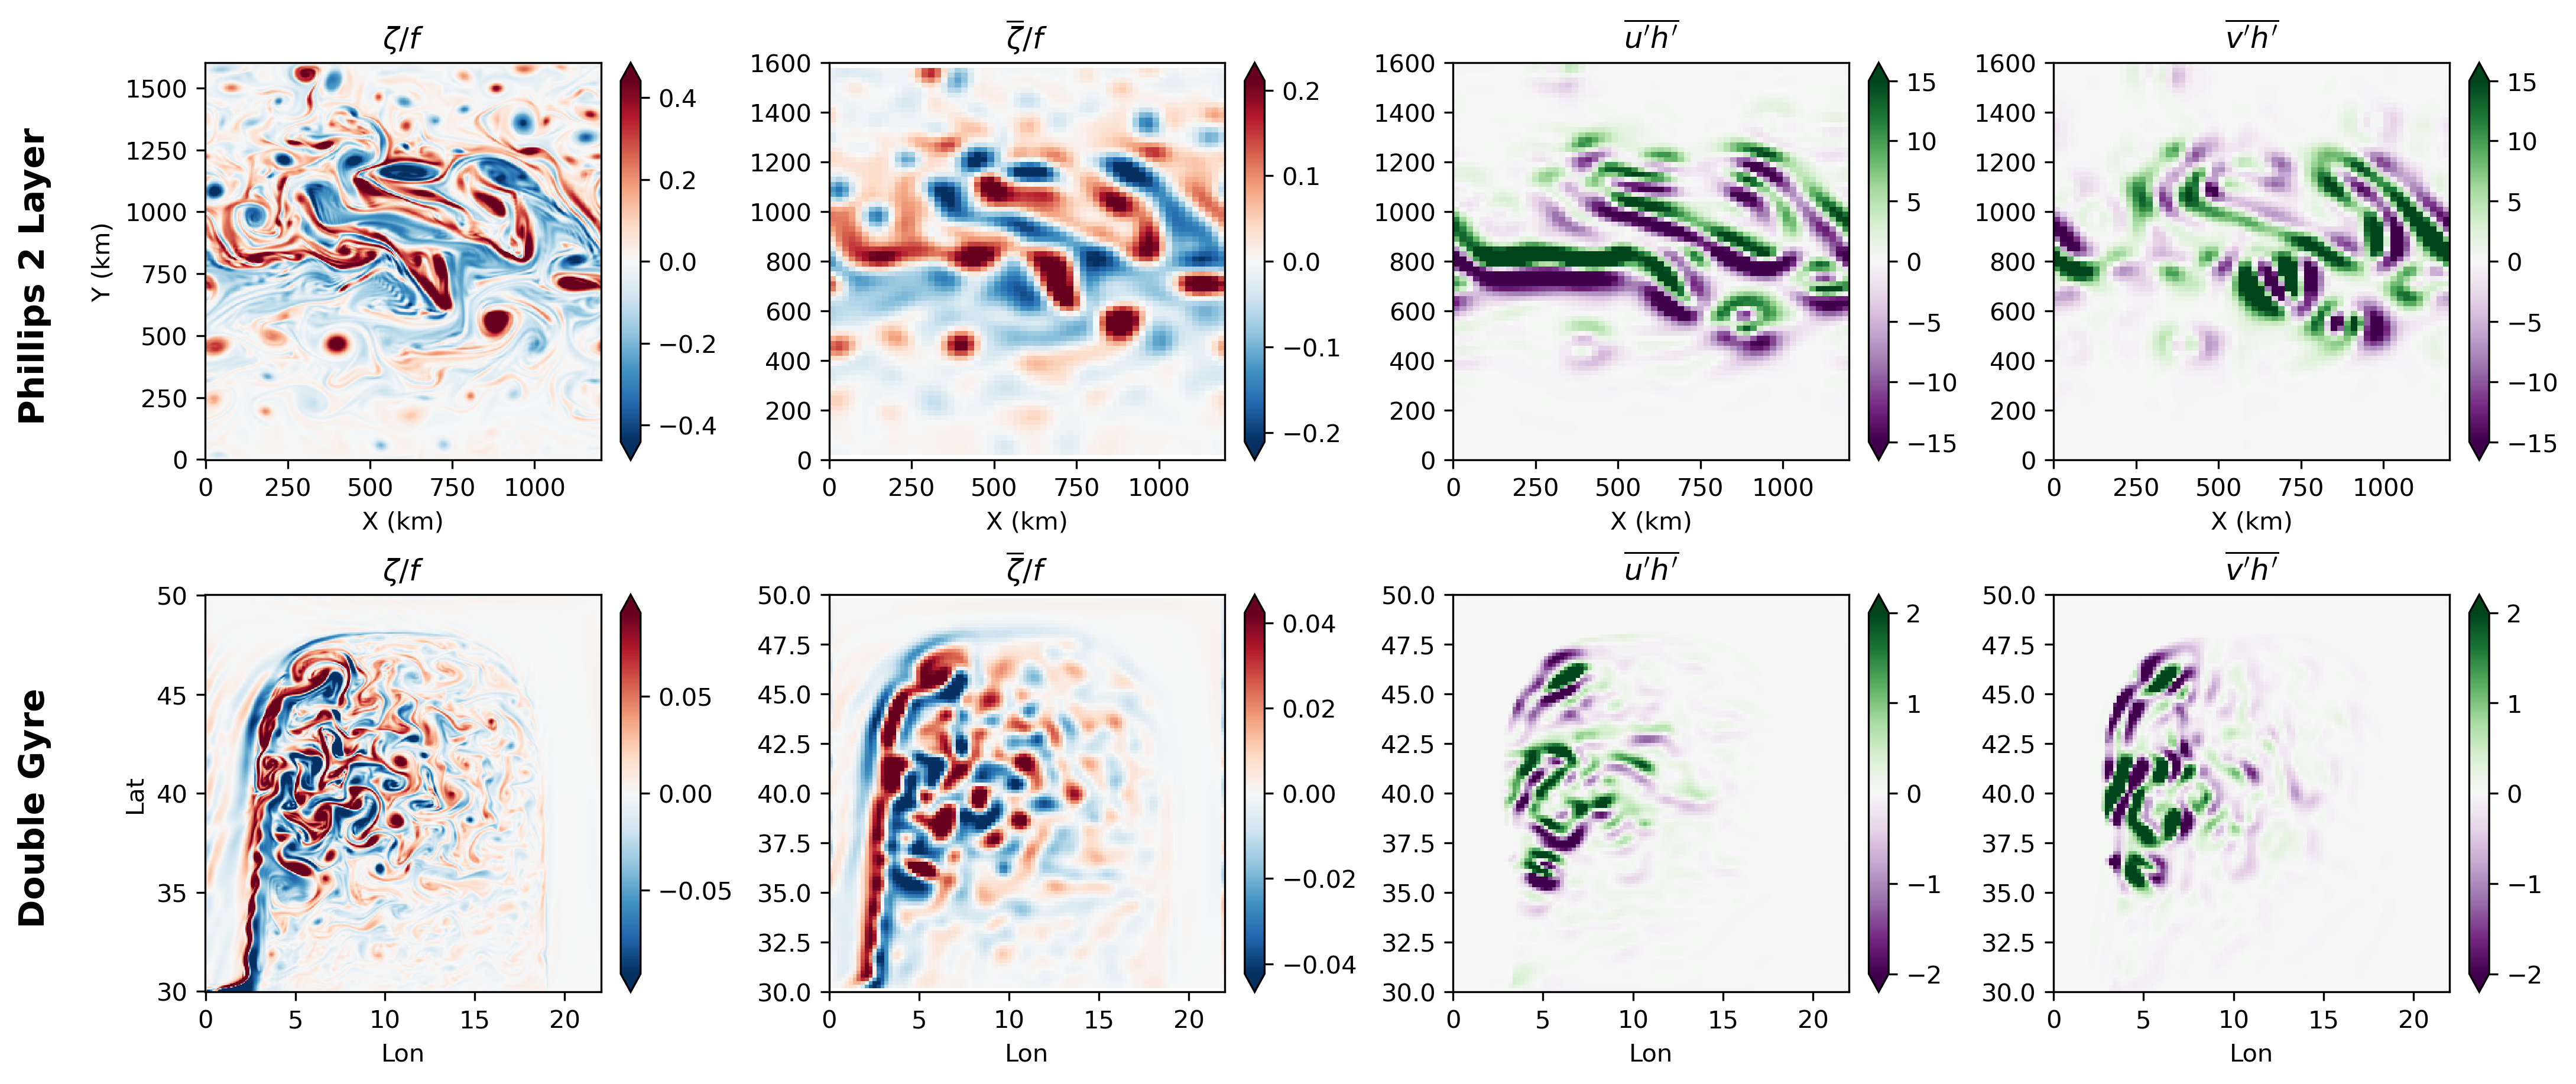
\includegraphics[width=\textwidth]{figures/Figure1.png}
\caption{Snapshots exemplifying the high-resolution vorticity (left), filtered vorticity (second column), and sub-grid fluxes (last two columns) from the Phillips 2 layer (top) and Double Gyre (bottom). The filtered fields are shown from the case of coarse-graining scale of 20~km. Only the upper layer data is shown, and different panels have different color ranges. }
\label{fig:intro_panels}
\end{figure}


\begin{figure}
\noindent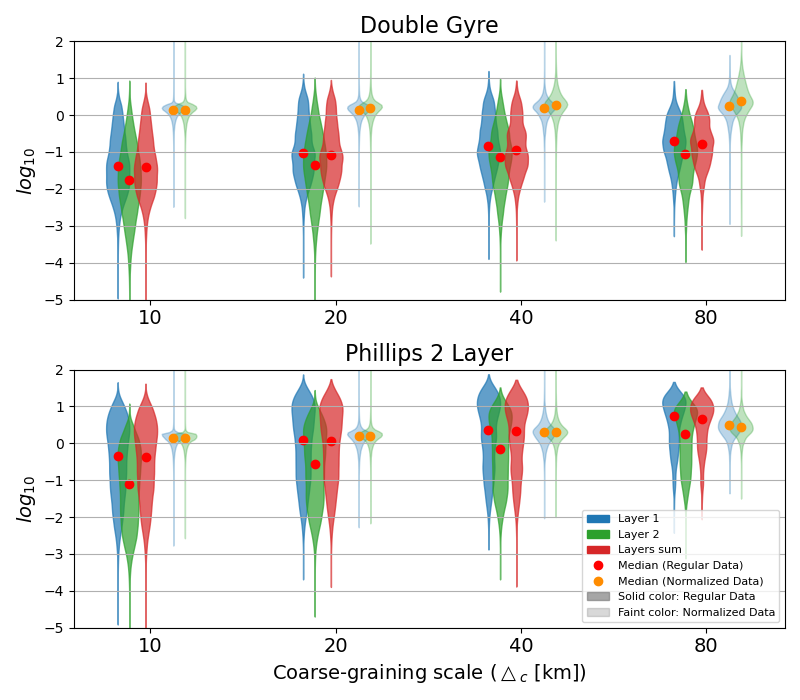
\includegraphics[width=\textwidth]{figures/Figure2.png}
\caption{\textbf{Distribution of output data:} Distributions of the logarithm of the thickness flux magnitudes ($|\mathbf{F}_n|$) in both layers and their sum (barotropic contribution), and the normalized thickness flux ($\frac{|\mathbf{F}_n|}{\, \triangle_c^2 |\nabla \overline{\mathbf{u}}_n||\nabla \overline{h}_n|}$) in both layers for the different experiments (top and bottom panel) and different coarse-graining scales (indicated on the x-axis). The legend in the lower panel is used to indicate the different elements in both the panels. The density of the distribution is indicated by the width of each patch, with wider regions, usually in the middle, indicating a higher concentration of data points near those values.  }
\label{fig:dist_outputs}
\end{figure}

\begin{figure}
\noindent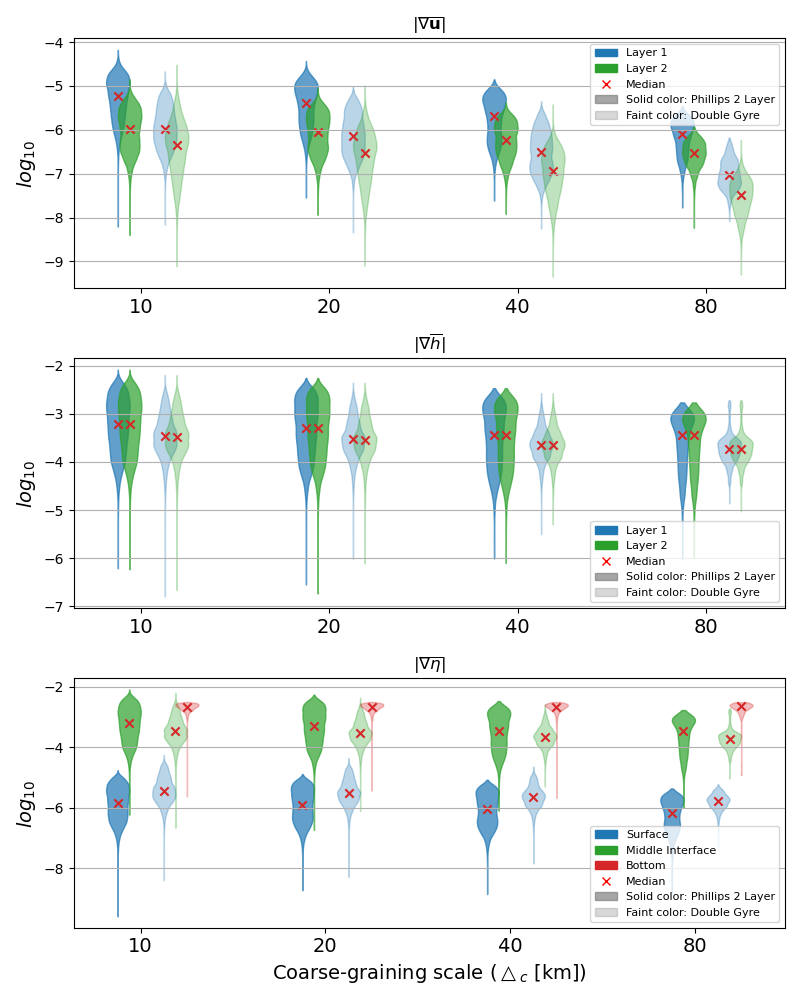
\includegraphics[width=\textwidth]{figures/Figure3.png}
\caption{\textbf{Distribution of input data:} Distributions showing the logarithmic magnitude range of different filtered fields, which may be used as input variables for neural network design from both simulations and at different layers and interfaces. Similar to Figure \ref{fig:dist_outputs} the width of the patch corresponds to values with a higher probability of occurence.}
\label{fig:dist_inputs}
\end{figure}


\begin{figure}
\noindent\includegraphics[width=\textwidth]{figures/maps_ML_skill.png}
\caption{The true (1st column), predicted (2nd column), and prediction error (3rd column) in the along (1st and 3rd row) and across (2nd and 4th row) thickness gradient fluxes for the top (1st and 2nd row) and bottom (3rd and 4th row) layers of the Double Gyre simulations. Here the results are shown for the ML model of the following configuration: 3X3 stencil, trained on data from DG+P2L, and $5090$ learnable parameters. These offline skill results are shown for the filter scale of $100$km. Note that the prediction error has been multiplied by a factor of 5 to be easily visible on the same scale as the true and predicted fluxes.}
\label{fig:poitwise_prediction_maps}
\end{figure}

\begin{figure}
\noindent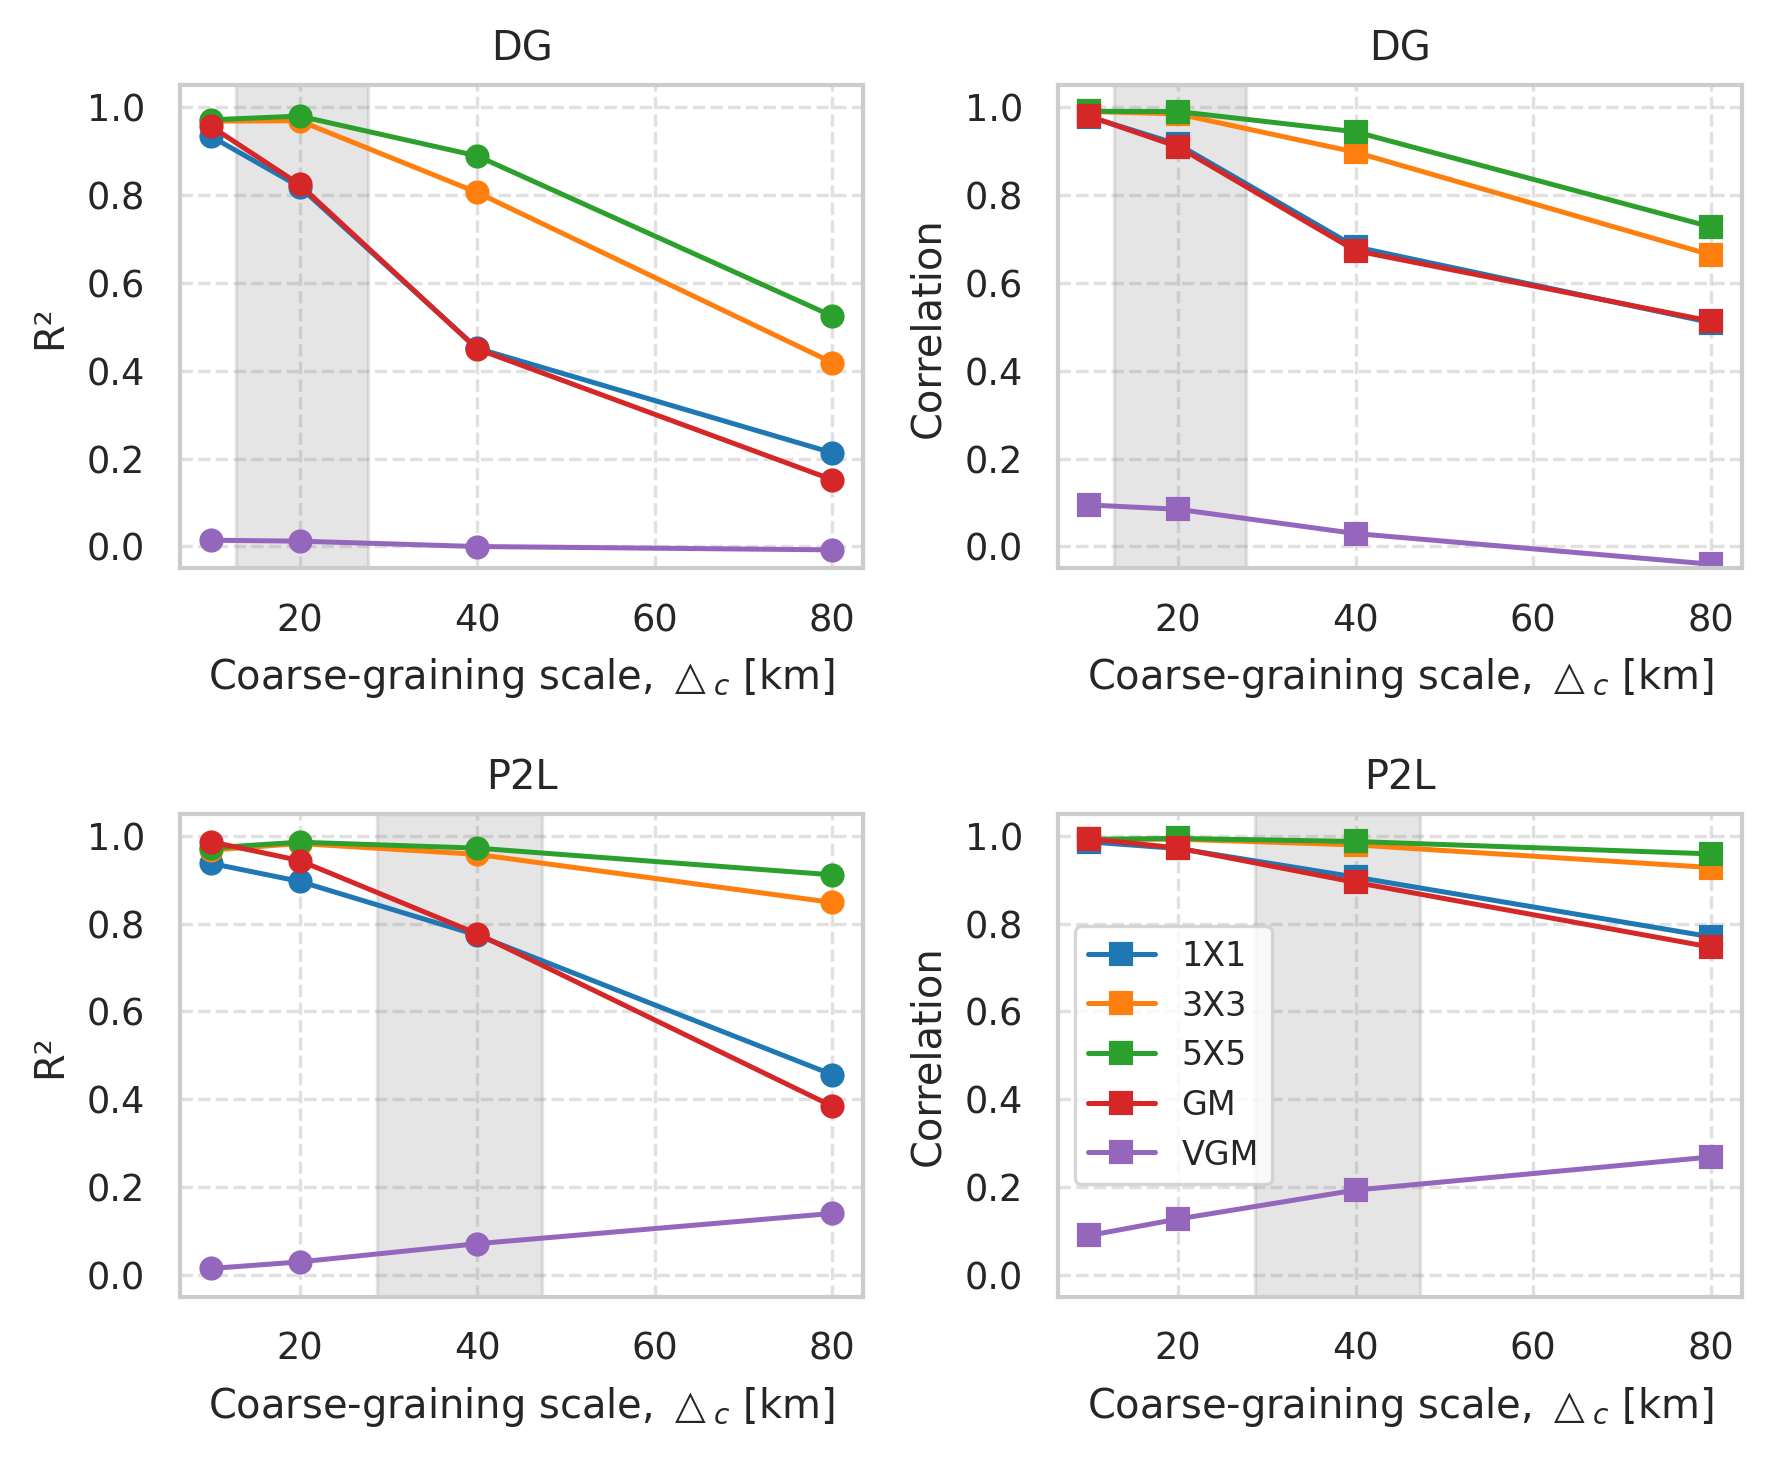
\includegraphics[width=\textwidth]{figures/skill_metrics_plot.png}
\caption{Pointwise offline skill in terms of the R2 skillscore (left column) and correlation (right column) for 5 different models (indicated in the legend) at different scales (x-axis) and in the double gyre (top) and Phillips 2 layer (bottom) simulations. The metrics were evaluated over both layers and across the full test dataset spanning X years. The gray shaded area indicates the deformation radius range (10 to 90$^{th}$ percentile) in the simulation.}
\label{fig:pointwise_skill}
\end{figure}

\begin{figure}
\noindent\includegraphics[width=\textwidth]{figures/R2_Corr_combined_plot_bulk.pdf}
\caption{Offline skill in predicting the time average of the subgrid fluxes, using five different models (columns). 
For all models the skill in predicting the time averaged flux is quantified as the average skill over the two layers and for both the along and across thickness gradient direction. 
%For the Gent-McWilliams model the skill is taken as the average between the along and across thickness gradient fluxes. 
}
\label{fig:bulk_skill}
\end{figure}

\begin{figure}
    \centering
    \includegraphics[width=\linewidth]{figures/RV_main_models.png}
    \caption{Snapshots of relative vorticity and the EKE spectra from different Phillips 2 layer simulations discussed in section 4.2.
    Note that the colorbar on the bottom right panel has been adjusted to show the range of values in that simulation. }
    \label{fig:P2L_RV}
\end{figure}


\begin{figure}
    \centering
    \includegraphics[width=\linewidth]{figures/stacked_energy_panels_P2L.png}
    \caption{Bulk metrics to evaluate the online skill of the parameterizations in different experiments of Phillips 2 layer simulation (indicated along the x-axis). (a) Peak value of the total meridional transport in the upper layer for the resolved, parameterized and sub-filter components. (b) Kinetic energy and (c) available potential energy of the mean and eddy flow coming from the resolved and subgrid contributions. (d) The impact of the parameterized or subgrid fluxes on the mean and eddy APE tendency; no bar plot is shown for the high-resolution simulation as in this instance there are no sub-grid or parameterized thickness flux.  }
    \label{fig:P2_all_panels}
\end{figure}



\begin{figure}
    \centering
    \includegraphics[width=\linewidth]{figures/mean_SSH_logKE_combined.png}
    \caption{Mean SSH (top row) and EKE (bottow row) the for the Double gyre simulations discussed in section 4.3. The RMSE in the SSH and middle interface height are indicated for the three $1/5^o$ resolution simulations.}
    \label{fig:DG_maps}
\end{figure}

\begin{figure}
    \centering
    \includegraphics[width=0.9\linewidth]{figures/energy_budget_DG.png}
    \caption{The volume integrated KE (top) and APE (bottom) for the Double Gyre simulations (indicated along x-axis) discussed in section 4.3. The mean, eddy, and sub-filter contributions are indicated. }
    \label{fig:DG_energy}
\end{figure}

\begin{figure}
    \centering
    \includegraphics[width=\linewidth]{figures/APE_tend_DG.png}
    \caption{APE tendency exerted on the mean (top) and eddy (bottom) APE by the sub-grid or parameterized fluxes in the Double Gyre simulations discussed in section 4.3. The volume integrated value for each panel is indicated at the top left.  }
    \label{fig:DG_APE_tend}
\end{figure}

%%%%%%%%%%%%%%%%%%%%
%%%% Appendix %%%%%%%
%%%%%%%%%%%%%%%%%%%%
\appendix

%%%%
%%%%
% \section{Simulation details}
% \label{app:sim_details}
% We used data from two idealized high resolution simulations in this work.
% \subsection{Phillips 2 layer - MOM6}
% Refer to \cite{hallberg2013using}.

% \subsection{Double gyre - MOM6}
% Refer to \cite{zhang2023implementation}.

%%%
\section{Offline Skill Metrics}
\label{app:offline_skill_metrics}
% Mean square error is used as the loss function
% \begin{equation}
%     MSE = \overline{(y - \hat{y})^2}
% \end{equation}
% Here the average is taken over all outputs (two directions of the SGS flux), and all samples.

To evaluate the skill of our ML model in an offline setting we use two main skill metrics. The first is the coefficient of determination or R2 skill, defined as, 
\begin{equation}
    R^2 = 1  - \frac{\overline{(y - \hat{y})^2}}{\overline{(y - \overline{y})^2}},
\end{equation}
$y$ is the truth value and $\hat{y}$ is the prediction. The $\overline{(\cdot)}$ corresponds to average over all samples being considered, which is chosen to be over both flux components from both layers, full spatial domain, and all temporal snapshots in the test data (unless indicated otherwise). The R2 skill will be 1 when prediction is perfect and reduces as prediction gets worse. 

The second metric is the Pearson correlation coefficient, 
\begin{equation}
    C = \frac{\overline{(y - \overline{y})(\hat{y} - \overline{\hat{y}})}}{\sqrt{\overline{(y - \overline{y})^2}\overline{(\hat{y} - \overline{\hat{y}})^2}}},
\end{equation}
which is 1 when the truth and the prediction are perfectly correlated, -1 for inverse correlation, and 0 for no correlation.

%The relative error in spectral space is defined as :
%...



\section{Eddy driven stream function}
\label{app:eddy_streamfn}

The SGS thickness flux corresponds to a volume flux in a layer ($\mathbf{F}_n$), and the net SGS volume flux below a certain interface can be represented as a stream function \cite{mcdougall2001temporal}: 
\begin{equation}
    \mathbf{\Psi}_{n-1/2} = \sum_{i=N}^n \mathbf{F}_i. %(\overline{\mathbf{u}_i h_i} -  \overline{\mathbf{u}}_i \overline{h_i}),
\end{equation}
Inversely, the SGS thickness flux in any layer can be expressed in terms of these SGS stream function as:
\begin{align}
    \mathbf{F}_n & =  \overline{\mathbf{u}_n h_n} -  \overline{\mathbf{u}}_n \overline{h_n} \\
    %& = \overline{\mathbf{u}_n (\eta_{n-1/2} - \eta_{n+1/2})} -  \overline{\mathbf{u}}_n \overline{(\eta_{n-1/2} - \eta_{n+1/2})} \\
    & = \mathbf{\Psi}_{n-1/2} - \mathbf{\Psi}_{n+1/2} \\
    &  = \delta_n \mathbf{\Psi} \\ 
\end{align}
This streamfunction represents a 2D divergent bolus velocity, $\mathbf{u}_n^* = \delta_n \mathbf{\Psi}/\overline{h_n}$.

While we have presented the problem entirely in terms of thickness fluxes to be used in layered models (section 2), a comparable representation of SGS buoyancy fluxes in terms of a stream function can be done for depth-level models. When representing the SGS buoyancy fluxes in depth-level models, a 3D non-divergent velocity field is constructed using this streamfunction - the quasi-stokes velocity - with no-flow boundary conditions at the top and bottom may be used.  

\section{Interface Diffusion and Gent-McWilliams (GM) Parameterization}
\label{app:GM_param}
This SGS thickness flux in MOM6 is parameterized by the interface diffusion parameterization, which prescribes the eddy driven streamfunction as,
\begin{equation}
    \mathbf{\Psi}^{GM}_{n-1/2} = - \kappa^{GM} \nabla \eta_{n-1/2}, \quad 2 \leq n \leq N.
    \label{eqn:GM_streamfunction}
\end{equation}
% and the corresponding thickness flux would be: 
% \begin{equation}
%     \mathbf{F}^{GM}_{n} = - \kappa^{GM}_{n-1/2} \nabla \eta_{n-1/2} + \kappa^{GM}_{n+1/2} \nabla \eta_{n+1/2},
%     \label{eqn:GM_thickness_flux}
% \end{equation}
In this scheme, the stream function at the top and bottom of the water column are prescribed to be zero ($\mathbf{\Psi}^{GM}_{1/2} = \mathbf{\Psi}^{GM}_{N+1/2} = 0$), which ensures that the sub-grid thickness fluxes do not result in any barotropic SGS volume transport. This parameterization always flattens isopycnal surfaces and reduces APE.  

This parameterization is a close cousin of the Gent-McWilliams parameterization \cite{gent1990isopycnal, gent1995parameterizing}, which is designed for use in z-level models, and also reduces APE of the resolved state. 

%In reality, none of these parameterization assumptions may be completely accurate, and the goal of our work is to improve on this parameterization of sub-grid flux. Here we will use a neural network to parameterize $\mathbf{\Psi}_{n-1/2}$. 

%\textcolor{red}{The assumption of zero $\mathbf{\Psi}$ at the top and bottom is only technically defensible in the interpretation of the coarse resolution model as being representative of the TWA equations mapped to mean depth coordinates. In stacked shallow water model, the natural boundary conditions are of zero streamfunction at vertical side boundaries \cite{killworth2001boundary}.}



%%%%
\section{Velocity Gradient Model (VGM)}
\label{app:VGM}

The velocity gradient model is a structural model, where the goal is to accurately predict the patterns in the SGS forcing.  It is derived based on a Taylor series expansion, and by keeping only the first term of the expansion (see derivation in \citeA{aluie2022effective} or appendix B of \citeA{khani2023gradient}). 


For thickness fluxes, the VGM predicted flux is: 
\begin{equation}
    \mathbf{F}_n^{VGM} = C_{VGM} \triangle_c^2 \nabla \overline{\mathbf{u}}_n \nabla \overline{h}_n
\end{equation}
where 
\begin{equation}
    \nabla \overline{\mathbf{u}}_n = 
    \begin{bmatrix}
        \partial_x \overline{u}_n & \partial_y \overline{u}_n \\
        \partial_x \overline{v}_n & \partial_y \overline{v}_n \\
    \end{bmatrix},
\end{equation} 
\begin{equation}
    \nabla \overline{h}_n = 
    \begin{bmatrix}
        \partial_x \overline{h}_n \\
        \partial_y \overline{h}_n \\
    \end{bmatrix},
\end{equation}
$\triangle_c$ is a coarse-graining scale, and $C_{VGM}$ is a scaling coefficient corresponding to the filter scale. Note that in the presence of topography, we defined our filters such that $\overline{\eta}_b = \eta_b$. So, the sub-grid thickness flux in the bottom layer is just the sub-grid deformable thickness flux. 

Unlike the GM parameterization, the VGM based expression is not guaranteed to the APE reducing, and the impact depends non-linearly on the resolved flow.
%, and so $\mathbf{F}_n^{VGM} = c \triangle^2 \nabla \overline{\mathbf{u}}_n \nabla \overline{h}_n^{deformable}$.

% For calculating the eddy driven stream function, we will need to sum over layers: 
% \begin{equation}
%     \mathbf{\Psi}_{n-1/2} = \sum_{i=N}^n c \triangle^2 \nabla \overline{\mathbf{u}}_i \nabla \overline{h}_i^{deformable},
% \end{equation}
% which is not necessarily zero at the surface. 



%%%%
\section{Rotation to thickness gradient frame}
\label{app:frame_rotate}
In this work we often rotate all directional quantities: SGS flux vectors, the velocity gradient tensor and all thickness gradients, to a thickness gradient frame. 
This thickness gradient frame is defined using a set of orthogonal vectors in the horizontal plane. The first of these vectors,
\begin{equation}
    \hat{\mathbf{T}} = \frac{\nabla \overline{h}_n}{|\nabla \overline{h}_n|} = \frac{\partial_x \overline{h}_n}{|\nabla \overline{h}_n|} \mathbf{\hat{i}} + \frac{\partial_y \overline{h}_n}{|\nabla \overline{h}_n|} \mathbf{\hat{j}},
\end{equation}
points down the thickness gradient. The orthogonal (second) vector, following the right hand rule, is defined as, 
\begin{equation}
    \hat{\mathbf{N}} = \mathbf{\hat{k}} \times \frac{\nabla \overline{h}_n}{|\nabla \overline{h}_n|} = \frac{-\partial_y h_n}{|\nabla \overline{h}_n|} \mathbf{\hat{i}} + \frac{\partial_x h_n}{|\nabla \overline{h}_n|} \mathbf{\hat{j}}.
\end{equation}
The corresponding rotation matrix is defined as
\begin{equation}
    \mathbf{R}_n = 
    \begin{bmatrix}
        \hat{\mathbf{T}} & \hat{\mathbf{N}}
    \end{bmatrix} = 
    \frac{1}{|\nabla \overline{h}_n|}
    \begin{bmatrix}
        \partial_x \overline{h}_n & - \partial_y \overline{h}_n \\
        \partial_y \overline{h}_n & \partial_x \overline{h}_n \\
    \end{bmatrix}.
\end{equation} 

This matrix can be used to rotate vector components and tensor components into the thickness gradient frame. Example, the SGS flux vector components in rotated frame can be diagnosed as 
\begin{equation}
    \widetilde{\mathbf{F}_n} = \mathbf{R}_n^T \mathbf{F}_n,
    \label{eqn:vec_rot}
\end{equation}
and the velocity gradient tensor components in  can be rotated as, 
\begin{equation}
    \widetilde{\nabla \overline{\mathbf{u}}_n} = \mathbf{R}_n^T (\nabla \overline{\mathbf{u}}_n) \mathbf{R}.
\end{equation}

When the operation in Equation \ref{eqn:vec_rot} is applied to the thickness gradient itself, we get the expected result 
\begin{equation}
    \widetilde{\nabla \overline{h}_n} = |\nabla \overline{h}_n| \hat{\mathbf{T}} + 0 \hat{\mathbf{N}},
\end{equation}
since this vector does not have any projection orthogonal to the thickness gradient direction by definition.



%(\textcolor{red}{Does this mean that we can make some error in F1, and things will still go fine for PE}.)


\section{ML Model Design Sensitivity}
\label{app:ML_model_sensitivity}
There is a vast range of design choices that need to be made when working with machine learning models and designing parameterizations. For example there can be sensitivity and interdependence on (i) ML model size and architecture (e.g. we chose MLP here), (ii) training data size, (iii) training data source (which idealized simulation is used to train), (iv) learning rate and optimizers, (v) random parameter initialization, (vi) training targets, (vii) norms optimized in loss functions, (viii) input stencil/ domain of influence, (ix) selection of input features etc. It is infeasible to do a complete search over the entire parameter space and some human intuition is often used to guide the design, here we show the impact of some choices that helped guide our decisions. 
%During the initial design development process few choices were randomly sampled, and appropriate changes were made based on human intuition. Some of these choices were then rigorously tested, as shown below.
%%%%
%The design of the model features helps us build our physical knowledge and intuition, and also preconceived biases, into our ML model. 
%In preparation for this study, we tested a wide range of models, as listed here: 
% \begin{itemize}
%     \item $\mathbf{F} = f(\nabla u, \nabla h, \triangle)$ Raw model
%     \item $\mathbf{F}' = f(\nabla u', \nabla h', \triangle)$ Coordinate invariant model
%     \item $\mathbf{F}' = \triangle^2 |\nabla u| f(\nabla u'/|\nabla u|, \nabla h'/|\nabla h|, |\nabla h|)$ Coordinate invariant with non-dimensionalized and range limited inputs
%     \item $\mathbf{F}' = \triangle^2 |\nabla u| f(\nabla u'/|\nabla u|, \nabla h'/|\nabla h|) g(|\nabla h|)$ Coordinate invariant with non-dimensionalized and range limited inputs, and assuming a separable model
%     \begin{itemize}
%         \item $g(|\nabla h|) = |\nabla h|^\alpha$, $\alpha=1$ Polynomial form.
%         \item $g(|\nabla h|)$ is learnt.
%     \end{itemize}
% \end{itemize}

%\textbf{Raw Model} This model is relatively simple. However, it struggles to work across filter scales and layers, since the output data varies quite significantly in magnitude and the loss function will end up not being able to learn properties for the data that is in the smaller range of values. \textbf{Coordinate invariant model} The behavior of this model is similar to the raw model, since the range variability of outputs is still quite large. 

\subsection{Impact of different network sizes}
\label{app:ML_model_sensitivity/size}
We want the most skillful predictions at the lowest cost (least number of operations per evaluation of the MLP). We expect that the skill will increase with increasing the number of trainable parameters, but likely saturate beyond a certain point as there may be no more predictive power in the input features left to be extracted. 
In Figure \ref{fig:compare_model_size} we quantify this behavior for one particular class of models (these were trained with following choices: trained using data from the double gyre experiment, where all the data was rotated to the thickness gradient frame. Non-dimensional velocity and thickness gradients were used as inputs. Mean absolute error was used for the loss, with dimensional fluxes (equation 4) as output targets. Both inputs and outputs were normalized using order of magnitude estimates. We used the model snapshots 0-640 for training, 672-736 for evaluation and 736-800 for testing. Adam optimizer was used with a learning rate of 0.01, and training was continued till the relative improvement in the loss saturated within a relative tolerance of 0.01 (1\% error) for at least 10 epochs). 

The model skill, measured as the R2 value, improves as the number of parameters increase, and this is particularly apparent at larger filter scales and when the model stencil is wider. However, since skill is already very high at filter scales of 50 and 100~km this effect is minor, and at larger filter scales the skill seems to asymptote to its maximum value approximately around $10$K parameters.


\begin{figure}
\noindent\includegraphics[width=0.8\textwidth]{figures/comparing_model_sizes_across_scale.pdf}
\caption{ML model skill, defined as the R2 value, as a function of number of parameters for different filter scales. The details ML model being tested is described in \ref{app:ML_model_sensitivity/size}.}
\label{fig:compare_model_size}
\end{figure}


\subsection{Impact of training data size}
To test the impact that the amount of training data has, we experimented with the same setup as the one used in the previous section with varying amount of data. We fixed all aspects, and performed the test in the case where the stencil size is 3X3 and ML model has 3386 parameters (model shape 54,36,36,2). 
We created batches of 16 model snapshots, and tested the effect that increasing the number of batches had. As shown in Figure \ref{fig:impact_training_data} the model skill increases up to about 128 batches (2048 model snapshots), but saturates past that point. This led us to use this data volume for training the model used in the main text.

\begin{figure}
\noindent\includegraphics[width=\textwidth]{figures/impact_training_data.pdf}
\caption{ML model skill, defined as the R2 value, as a function of filter scales for different number of data batches used for training.}
\label{fig:impact_training_data}
\end{figure}

\subsection{Impact of different loss functions and targets}
Non-dimensionalization of the sub-grid fluxes leads to a significant collapse in the distributions (see Figure \ref{fig:dist_outputs}), but also produces outliers (due to possibility of division by small velocity or thickness gradients). We have two choices of loss during training, either training on the dimensional fluxes $\mathcal{L}^{dim} = || \mathbf{F} - \mathbf{F}^{pred}|| = || \mathbf{F} - (\triangle^2|\nabla\mathbf{u}||\nabla h|) f_{\theta}(.)||$ or training on non-dimensional fluxes $\mathcal{L}^{non-dim} =  || \mathbf{F}/(\triangle^2|\nabla\mathbf{u}||\nabla h|) - f_{\theta}(.)||$. Both these forms should give us the same functional representation if a unique function $f_{\theta}(.)$ exists, but in the more realistic situation where $f_{\theta}(.)$ is an approximation and we want it to equally balance data coming from many regimes (different simulations, varying energy levels at different depths, etc) it would seem that $\mathcal{L}^{non-dim}$ might be a better choice. 
Along with this we also compared the use of mean square error (MSE) vs mean absolute error (MAE), since MAE is generally considered to be more tolerant to outliers. 

As seen in Figure \ref{fig:impact_loss_style}, the impact of these choices is relatively minor in the model considered in the previous section. Generally, the models trained using MAE seem to get better, except at the largest filter scales - where the model trained using non-dimensionalized outputs and MSE does better. However, this model is the worst performer at all other scales. The models trained using MAE also generally perform well across a wide range of scales (bottom panel). To our surprise, the impact of this choice was smaller than we had expected. For the main study we used $\mathcal{L}^{non-dim}$ along with MAE.


\begin{figure}
\noindent\includegraphics[width=\textwidth]{figures/impact_loss_style.pdf}
\caption{Top row shows the model skill in terms of R2 and correlation as a function of filter scale for different choices of loss function. Bottom two rows show the relative error, which is defined as the power spectrum of the (truth - prediction) divided by the power spectrum of the truth; value of greater than 1 implies that the variance in the anomaly field is greater than in the truth. 
}
\label{fig:impact_loss_style}
\end{figure}

\subsection{Impact of choice of training data}
We want to build ML models that are easily generalizable and training data agnostic. For example, a model trained on data from the P2L simulation should be able to make good predictions on data from DG experiment, and vice versa. Developing appropriate non-dimensionalizations, as highlighted in section 3, is a step in this direction. In Figure \ref{fig:impact_training_exp} we show that the model trained using data from both simulations simultaneously generally performs the best or close to the best, which is why we chose this training strategy for the model in the main text. 

It is worth noting that in fact even models trained on a single experiment, perform relatively well when tested on the other experiment. This is a result of the design choices we made. During the initial phase of our development, when we trained models to have the form of equation \ref{eqn:gen_ML_func}, the skill on unseen data was extremely poor (not shown), also see \citeA{perezhogin2025generalizable}.

\begin{figure}
\noindent\includegraphics[width=\textwidth]{figures/impact_training_exp.pdf}
\caption{Top two rows show the model skill in terms of R2 and correlation as a function of filter scale for different choices of training datasets. 
Bottom two rows show the relative error, which is defined as the power spectrum of the (truth - prediction) divided by the power spectrum of the truth; value of greater than 1 implies that the variance in the anomaly field is greater than in the truth. 
The title of the panels indicate the dataset on which testing is done, and the legend indicated the dataset that is used for training.}
\label{fig:impact_training_exp}
\end{figure}

\subsection{Impact of other aspects}

The random seed, which sets \textbf{the random initializations} of the ML model weights, seems to have a small impact on the skill. The model skill averaged across all filter scales, for the case discussed in the above section, varied between values of 0.7 - 0.725 over different random seeds. Since this effect seems small, in the main text we use only a single trained model. 


The \textbf{learning rate}, similarly has a minor impact on the final skill but impacts the nature of decrease in the loss. Large learning rates ($\sim 0.1$) lead to noisy training, while smaller rates ($<0.005$) take too many epochs to train. We found than a learning rate around 0.01 was optimal in not taking too many epochs and not being too noisy, which is what we used for the models discussed in the main text. 

\section{Simulation evaluation metrics}
\label{app:online_metrics}
Here we describe the metrics used to assess the physical properties of our simulations. 

\subsection{Overturning Circulation}
The overturning circulation ($\overline{V}_n (y)$) is defined as the volume transport across a longitude band in a particular layer,
\begin{equation}
    \overline{V}_n (y) = \oint \overline{v_nh_n}^t dx + \oint \overline{F^y_n}^t dx,
\end{equation}
where $F^y_n(x,y,z,t)$ is the sub-grid or sub-filter meridional flux in layer $n$, $\oint (.) dx$ corresponds to a zonal integral over the full longitudinal domain, and $\overline{(.)}^t$ indicates a time average. The first term on the RHS corresponds to the resolved overturning and includes the contribution from both the mean and the variable parts of the flow, and the second term corresponds to the parameterized overturning. 

\subsection{Eddy Kinetic Energy Spectrum}
The EKE spectrum provides an effective measure of the flow variability at different scales. 
Here, we define it as the zonal wavenumber ($k$) power spectrum of the $\mathbf{u}'_n(x,y,t) = \mathbf{u}_n(x,y,t) - \overline{\mathbf{u}}^t_n(x,y)$, 
\begin{equation}
    EKE_n(k) = \frac{1}{2}(\overline{|u'_n(k, y,t)|^2}^{t,y} + \overline{v'_n(k, y,t)|^2}^{t,y}),
\end{equation}
where $\overline{(.)}^{t,y}$ is a time and meridional average and $u'_n(k, y,t)$ is the zonal Fourier transform of $u'_n(x, y,t)$. By Parseval's theorem we have
\begin{equation}
    \sum_k EKE_n(k) = \frac{1}{2} \int ( \overline{u'_n(x, y,t)^2}^{t,y} + \overline{v'_n(x, y,t)^2}^{t,y}) dx,
\end{equation} 
which shows the scale-wise decomposition aspect of the zonal wavenumber EKE spectrum in the x-direction. We used the xrft package (\url{https://xrft.readthedocs.io/}) for this analysis.


\subsection{Integral Kinetic and Available Potential Energies}
The volume integrated KE in Joules is defined as: 
\begin{equation}
    KE = \frac{1}{2} \sum_k \int \rho_0 |\mathbf{u}_k|^2 h_k dx dy
\end{equation}
The $KE$ of the mean flow ($\overline{\mathbf{u}_k}^t$, $\overline{h_k}^t$) is referred to as $MKE$, and the $EKE$ is defined as $EKE = \overline{KE}^t - MKE$. 

The volume integrated APE in Joules is defined as: 
\begin{equation}
    APE = \frac{1}{2} \sum_k \int \rho_0   g'_{k-1/2} (\eta_{k-1/2} - \eta^{ref}_{k-1/2})^2 dxdy
\end{equation}

The $MAPE$ is the $APE$ of the mean state ($\overline{\eta_{k-1/2}}^t$), and the $EAPE$ is given by $EAPE = \overline{APE}^t - EAPE$

For filtered and coarsened flow ($\overline{\mathbf{u}_k}^{\triangle}$, $\overline{h_k}^{\triangle}$) we can also define the total kinetic energy ($KE^\triangle$), which has its corresponding mean ($MKE^\triangle$, for $\overline{\mathbf{u}_k}^{\triangle, t}$, $\overline{h_k}^{\triangle,t}$) and eddy ($EKE^\triangle$) components. Accordingly, we also define the SGS kinetic energies for the total ($KE- KE^\triangle$), mean ($MKE- MKE^\triangle$), and eddy ($EKE- EKE^\triangle$) flow. Similarly APE and its components can be defined for the filtered and coarsened flow and the SGS contribution.


\subsection{Available potential energy tendency due to sub-filter or parameterized fluxes}
\label{app:online_metrics/APE_tend}
Following \cite{loose2023comparing}, we can compute the impact that the SGS fluxes have on volume integrated APE tendency as, 
\begin{equation}
    (\partial_t APE)^{SF} = \sum_{n=1}^{N} \rho_0 \mathbf{F}_n \cdot \nabla M_n,
\end{equation}
where $\mathbf{F}_n$ are the SGS fluxes and $M_n$ is the dynamic pressure of the resolved. 

In a 2 layer fluid we  have, 
\begin{equation}
    (\partial_t APE)^{SF} = \rho_0 g^r_{1/2} (\mathbf{F}_1 + \mathbf{F}_2) \cdot \nabla \eta_{1/2} +  \rho_0 g^r_{3/2} \mathbf{F}_2 \cdot \nabla \eta_{3/2}.
\end{equation}
Notably, only the last term on the RHS, which arises due to SGS fluxes in the bottom layer, makes a significant contribution to the APE tendency, since $|\nabla \eta_{3/2}| >> |\nabla \eta_{1/2}|$. The barotropic contribution to APE, first term on RHS, is small. 

We decompose this tendency into the time mean and eddy contribution, by defining the contribution from the mean as  
\begin{equation}
    (\partial_t APE)^{SF, mean} = \rho_0 g^r_{3/2} 
 (\overline{\mathbf{F}_2}^t \cdot \nabla \overline{ \eta_{3/2}}^t),
\end{equation}
where the barotropic contribution is neglected. The eddy contribution is defined as $(\partial_t APE)^{SF, eddy} =\overline{(\partial_t APE)^{SF}}^t-(\partial_t APE)^{SF, mean}$.





\section{Online sensitivity to grid-size and parameterization coefficients}
\label{app:online_sensitivity}

Simulation of oceanic mesoscale turbulence is relatively sensitive to how well the first baroclinic deformation radius (shown in Figure \ref{fig:Rd} for the two simulations considered here) is resolved. In this study we chose our coarsening scale and simulation grid-size to lie in a range that encompasses the deformation radius, so that skill of the new parameterization at both the eddy permitting and non-eddying resolutions can be investigated. Here we provide details of the sensitivity of the coarse simulations to both grid spacing and parameterization coefficients. 

\subsection{Phillips 2 Layer}
For P2L simulation we tested the sensitivity of the overturning transport to the grid size and parameterization coefficients,  shown in Figure %\ref{fig:P2L_sensitivity} and 
\ref{fig:P2L_sensitivity_detail}. 

In this case, the unparameterized low resolution simulation always has lower overturning transport relative to the HR simulation. The response of the parameterized flux contribution to the GM diffusivity is almost linear and insensitive to grid size, and adjusting the GM diffusivity allows us to increase the total overturning transport to the appropriate value. However, this is only achieved when the diffusivity is relatively large ($\kappa_{GM}\sim 8,000-10,000\;m^2/s$), which is also a parameter regime in which the resolved eddying flow has been entirely suppressed. Consequently the contribution of the resolved flow to the overturning has been completely eliminated and the entire contribution comes from parameterized fluxes (Figure \ref{fig:P2L_sensitivity_detail} second column). There seems to be no lower diffusivity value at which the appropriate overturning can be achieved with only marginal impact to the resolved flow. 

In contrast, the simulations with the ANN based parameterization are usually able to achieve the appropriate level of overturning with minimal damage to the resolved flow. The response of the parameterized flux to the grid size and parameterization amplification coefficient ($C_{ANN}$) is non-linear. At grid sizes of 10 and 20~km, which are smaller than the deformation radius everywhere in the domain, the appropriate overturning is achieved at $C_{ANN}=1$ and with minimal damage to the resolved overturning. At a grid size of 80~km, which is larger than the deformation radius everywhere in the domain, the appropriate overturning is achieved at $C_{ANN}=2$. At the intermediate grid size of 40~km, the ANN parameterization does produce improvements to overall overturning with little damage to the resolved flow (also at $C_{ANN}=1$), but is unable to achieve similar overturning to the HR simulation. We anticipate that combining the thickness flux parameterization with a momentum flux parameterization may be able to produce further improvements at these intermediate resolutions. 



\subsection{Double Gyre}
Unlike the P2L simulation, in the DG case there is no overturning circulation. In the context of the thickness flux parameterization, the error in the MAPE is the most relevant, which is also linked to the error in mean SSH. We tested the sensitivity of these quantities and a few others to the parameterization coefficients and grid-size (Figure \ref{fig:DG_sensitivity}). 

For the GM parameterization, a diffusivity of about $200\;m^2/s$ is able to achieve the appropriate MAPE at all resolutions, which similar to the P2L also comes an almost complete damping of the resolved eddies. The ANN is able to achieve the best MAPE with $C_{ANN}\sim 0.5-0.75$, and this happens with relatively less deterioration in the resolved eddies.

\begin{table}[ht]
    \centering
    \renewcommand{\arraystretch}{1.2}
    \begin{tabular}{|c|cc|cc|}
        \hline
        $\triangle_c$ [km]
        & \multicolumn{2}{c|}{$\kappa_{GM}$ [m$^2$/s]} 
        & \multicolumn{2}{|c|}{$C_{VGM}$ [nondim]} \\
        \hline
        & \textbf{P2L} & \textbf{DG} & \textbf{P2L} & \textbf{DG} \\
        \hline
        10  & 137   & 40   & 0.110 & 0.075 \\
        20  & 596   & 105  & 0.077 & 0.072 \\
        40  & 2287  & 192  & 0.077 & 0.067 \\
        80  & 6266  & 108  & 0.091 & 0.048 \\
        \hline
    \end{tabular}
    \caption{Estimated GM diffusivity ($\kappa_{GM}$) and VGM coefficient ($C_{VGM}$) from the data using least squares fitting, for both the Phillips 2-Layer (P2L) and Double Gyre (DG) setups.}
    \label{tab:gm_vgm_estimates}
\end{table}




\begin{figure}
    \centering
    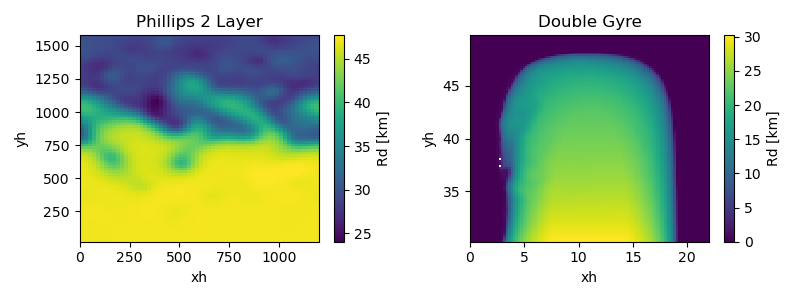
\includegraphics[width=\linewidth]{figures/SI_figures/Def_radii.png}
    \caption{First baroclinic deformation radii for P2L (left) and DG (right). Note the different range of scales for the two colobars.}
    \label{fig:Rd}
\end{figure}

% \begin{figure}
%     \centering
%     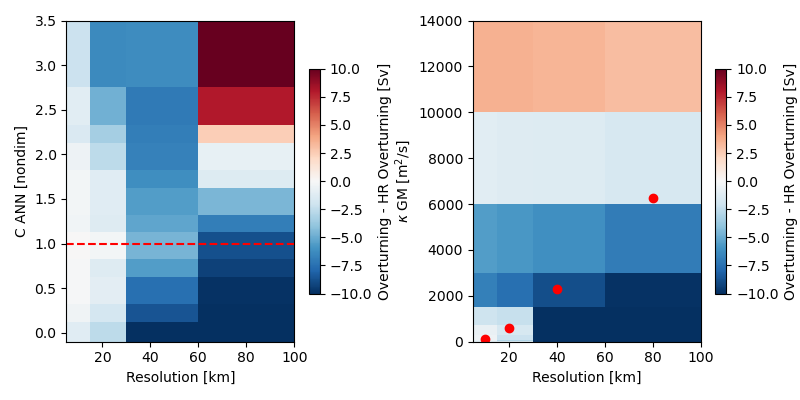
\includegraphics[width=1.0\linewidth]{figures/sensitivity_P2L.png}
%     \caption{Sensitivity of the overturning circulation to the MLP coefficient (left) and the GM diffusivity (right) for the Phillip 2 layer simulations at different resolutions. The dashed red line and red dots correspond to the optimal choice of these parameters suggested based on the offline analysis. }
%     \label{fig:P2L_sensitivity}
% \end{figure}

\begin{figure}
    \centering
    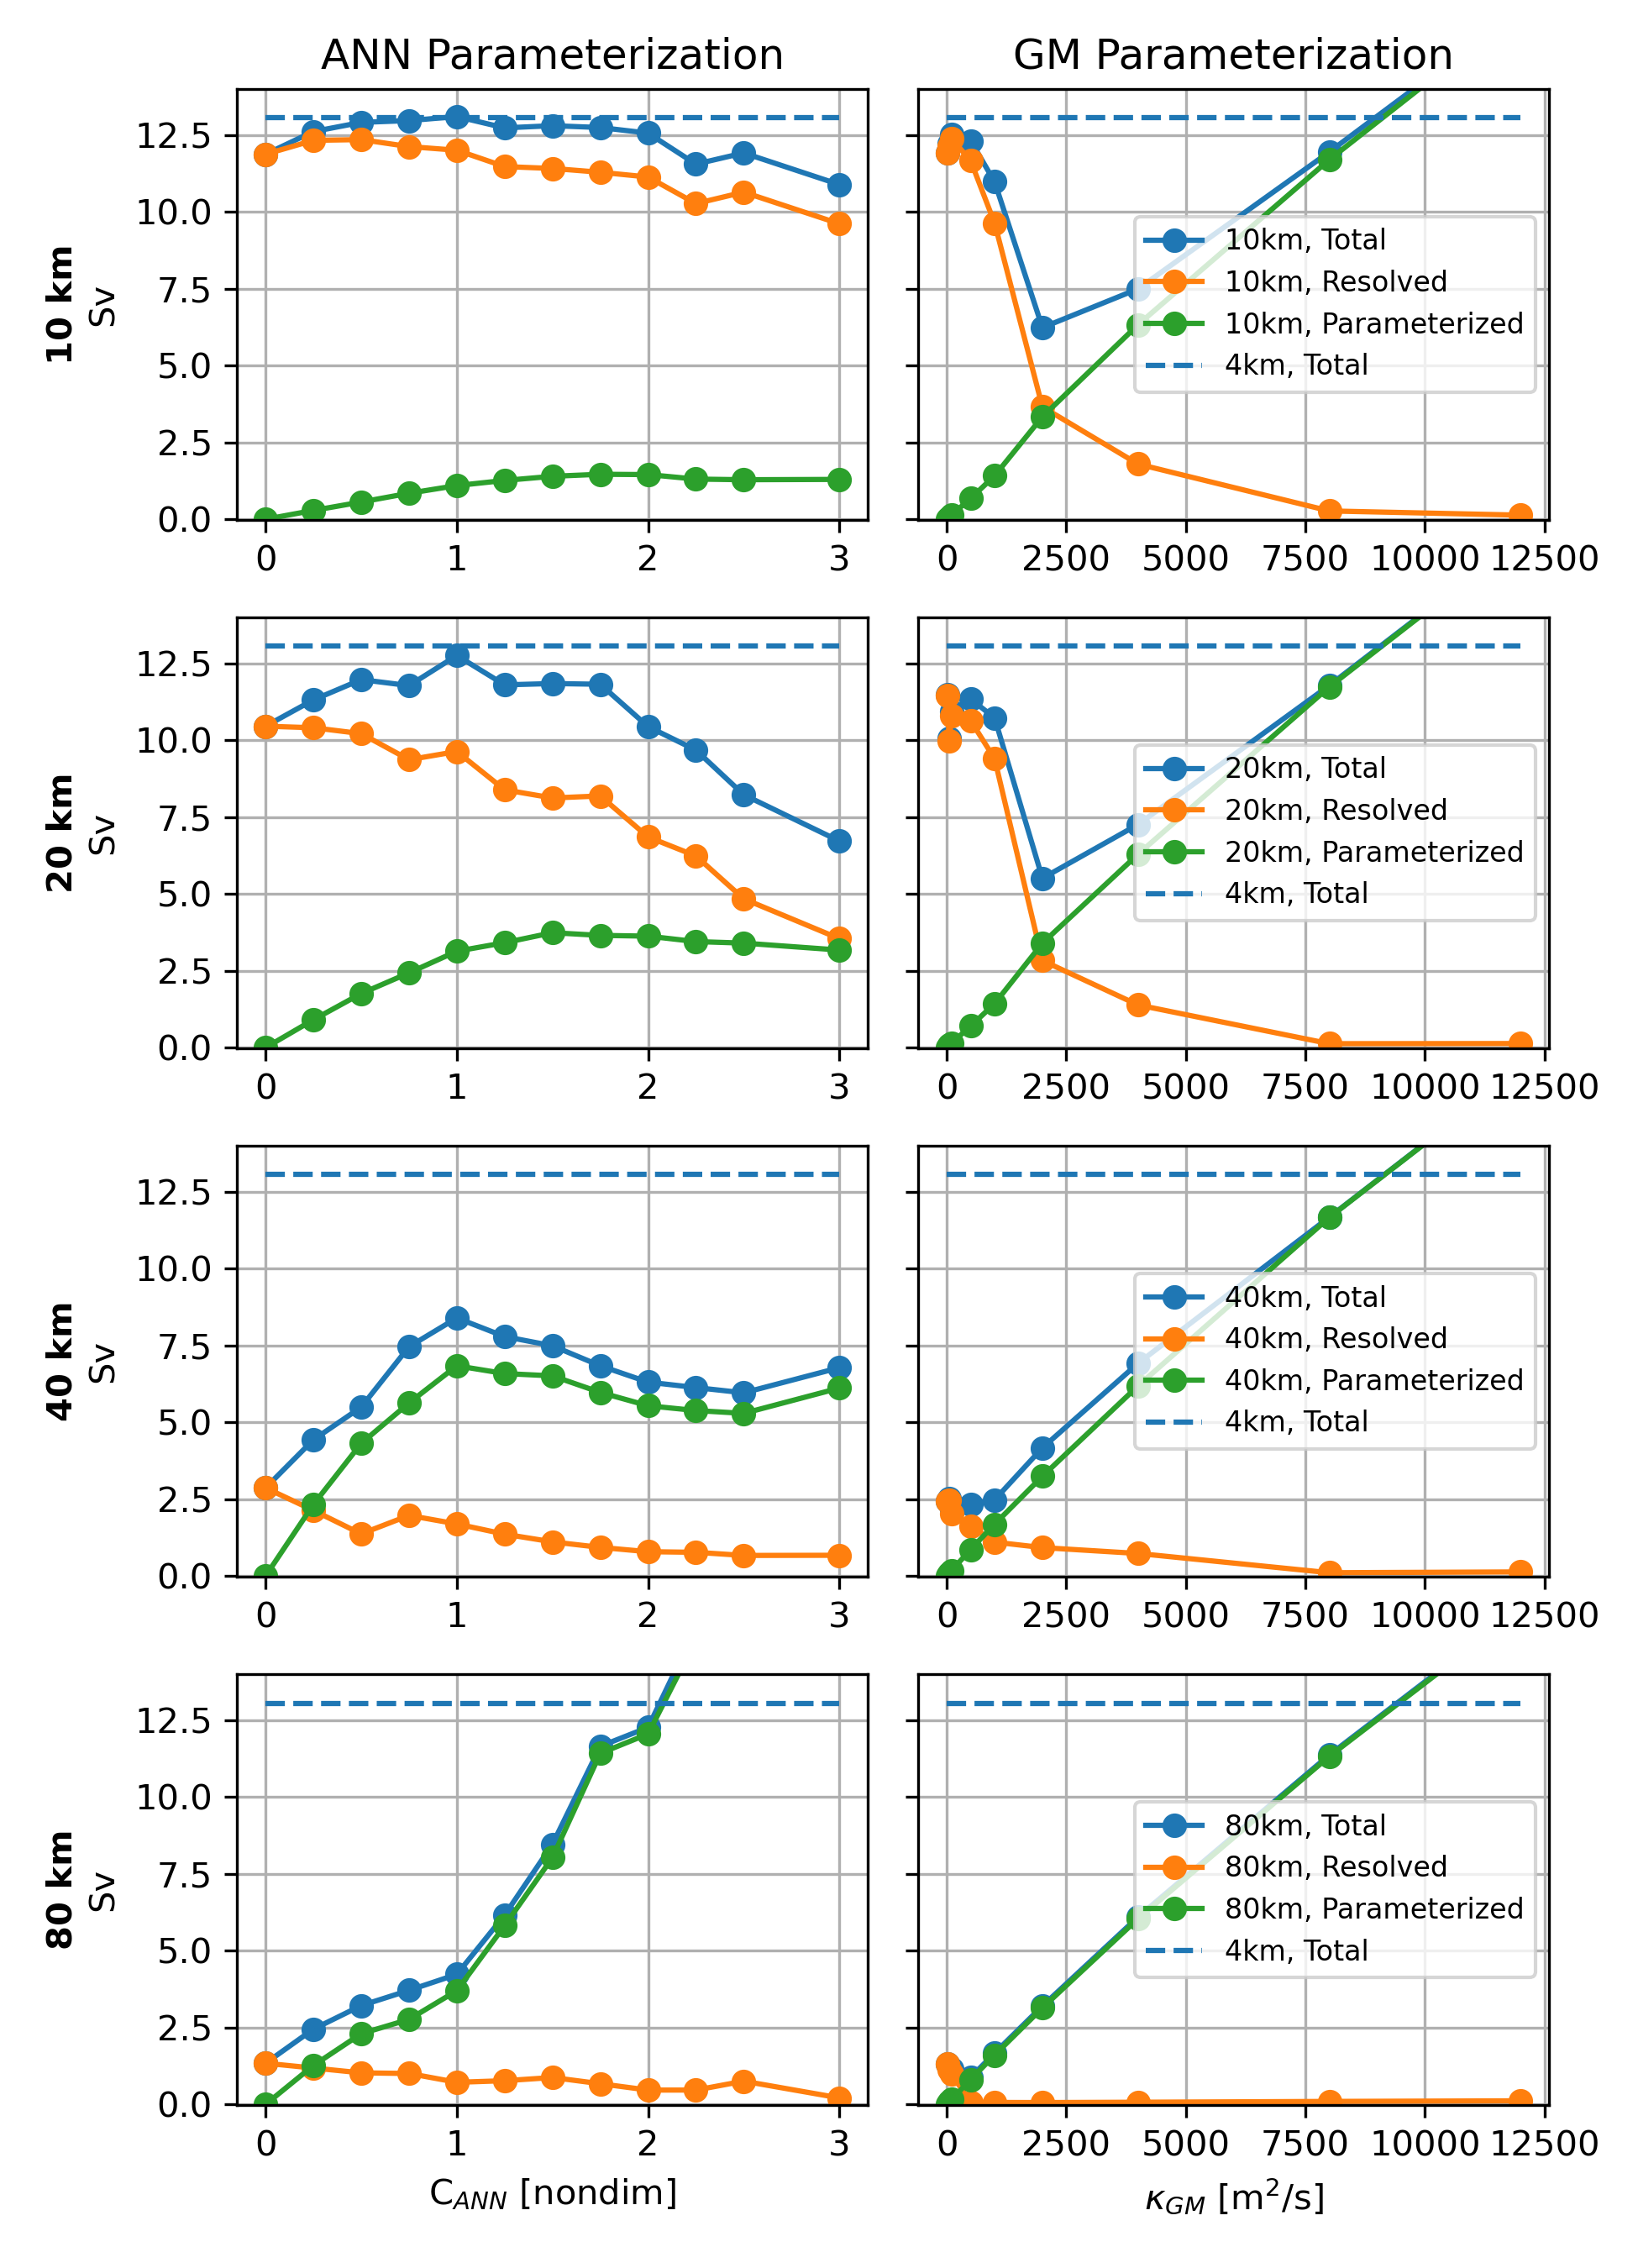
\includegraphics[width=\linewidth]{figures/sensitivity_P2L_multirow.png}
    \caption{Sensitivity of the overturning circulation and its resolved and parameterized components to the MLP coefficient (left) and the GM diffusivity (right) for the Phillip 2 layer simulations at different grid-sizes.}
    \label{fig:P2L_sensitivity_detail}
\end{figure}

\begin{figure}
    \centering
    \includegraphics[width=1.0\linewidth]{figures/SI_figures/DG_model_comparison.pdf}
    \caption{Sensitivity to the MLP coefficient (left) and the GM diffusivity (right) for the Double Gyre simulations at different resolutions.}
    \label{fig:DG_sensitivity}
\end{figure}













\bibliography{references}

\end{document}


\appendix 
\section{Data and Code Availability Statement}
%The data from the MITgcm channel simulation can be found on the Pangeo catalog (\url{https://catalog.pangeo.io/browse/master/ocean/channel/run_tracers_restored_zarr/}). 
The code for the analysis is available on github.



\section{Simulation details}

\subsection{Channel simulation - MITgcm}
During our initial explorations, we also used a dataset from a channel simulation using a Z-level MITgcm, fashioned to be an idealization of the Antarctic Circumpolar Current (ACC). The setup is the same as described in \cite{balwada2018submesoscale}, where the domain is a zonally periodic channel with a ridge, and the flow is forced by wind stress and surface buoyancy restoration. The resolution is 5km, which permits the development of an energetic mesoscale eddy field.

\subsection{Phillips 2 layer - MOM6}

\subsection{Double gyre - MOM6}



\section{Gent-McWilliams Parameterization}
\citeA{gent1990isopycnal} parameterizes the horizontal buoyancy fluxes as down-gradient diffusion
\begin{equation}
    \overline{u_i'b'} = - \kappa_{GM} \nabla \overline{b}
\end{equation}
where $\kappa_{GM}$ needs to be set appropriately.  It can chosen to be a constant (often varied according to grid resolution), constant but anisotropic (Bachman...), a simple function of the background state \cite{visbeck1997specification, ferreira2005estimating, danabasoglu2007effects}, or set according to sub-grid energetic constraints.

\subsection{GM in isopycnal coordinates}
There are two forms of the GM parameterizations, which is sometimes casually also referred to as thickness diffusion. 

The original one parameterization proposed by \citeA{gent1990isopycnal} effectively accounts for isopycnal interface diffusion. In this case the streamfunction is parameterized as, 
\begin{equation}
    \Psi = - K \nabla \eta,
\end{equation}
which results in a quasi-stokes advection of the form
\begin{equation}
    \mathbf{u}^* = \frac{\rho_0}{\overline{h}} \partial_{\rho} (K \nabla \eta).
\end{equation}

The alternative formulation is of thickness diffusion, 
\begin{equation}
    \mathbf{u}^* = - \frac{1}{\overline{h}}  -K \tilde{\nabla} h,
\end{equation}
where $\tilde{\nabla}$ corresponds to gradients taken along isopycnals. 

The two formulations are identical if the diffusion is depth-independent. 

Models usually take the first approach. This is due to a few advantages: (i) easier to impose boundary conditions so that the eddy-induced velocity does not contribute to the barotropic mode. This is equivalent to setting w=0 at top and bottom, which requires that the streamfunction be 0 (which is what naturally appears). This also ensures that the parameterization is not a source of momentum \cite{killworth1997parameterization}. (ii) McDougal and McIntosh argue that the uncertainty in B.C. can result in false overturning. [\textit{were some of these issues fixed by Ferrari et al 2010.}] (iii) Both schemes can reduce APE, but for the interface diffusion the reduction is local. [\textit{With the thickness diffusion scheme, the result can be an APE increase (imagine a layer sitting on topography. Similar things can also happen with PV diffusion, and does happen to some degree in the ocean [see \cite{marshall2012framework}]}.]

Now when it comes to using machine learning-based parameterizations, the last point is likely not relevant because the ML is not attempting to act like diffusion and in many instances, it does result in upgradient fluxes. 

\section{Baseline models}

\subsection{LES Gradient models}
A routinely used model in the large eddy simulation (LES) literature is a model based on a Taylor series expansion of the filtered fields. This provides a local expression.
\begin{equation}
    \overline{u_i'b'} = C_e \triangle_x^2 \frac{\partial u_i}{\partial x_j} \frac{\partial b}{\partial x_j}
\end{equation}

Where $C_e$ is set to 13/6. 
Note that since we only filter data horizontally, there is no vertical dependence in this expression. Such a model was first suggested in the LES community by \cite{leonard1975energy}, and more recent a priori applications to oceanographic regimes can be found in in \cite{aluie2022effective, khani2023gradient}. As shown in our results, the skill of this model deteriorates as the filter scale gets larger and starts to encompass scales larger than



\section{Impacts of averaging and assuming QG}
Here we evaluate how the assumptions impacted the sub-grid forcing ($S_{sg}$) and their impact on the energetics ($w'b'$).

...

\section{Hyperparameter tuning for ANN model}
...

Main lessons learnt from tuning inputs, arch size, etc.
\begin{itemize}
    \item Including inputs like vertical shear, vertical temp gradient does not significantly help the model. 
    \item For the ANNs usually there is a maximum model size upto which widening hidden layers or adding hidden layers helps, beyond that there are no gains (almost like a threshold beyond which there are minimal returns). 
    \item One would think that having no bias in the ANN should not be a problem, as we may want zero input to produce zero output. However, the training of models with no bias doesn't result in as high of a skill as when bias is included.
    
\end{itemize}

\section{Comparing ML models trained on single filter scale to model trained across a number of filter scales}
In our original experimentation, we trained models at particular filter scales, before expanding to the scale-aware model that has been described in the paper. Here we describe how the performance varies. 


\section{Coarsening operations for C-grid}

\section{Impact of training grid on performance}
The main results shown above were from a model which was trained by interpolating all the required inputs and outputs to the same center point. However, when implementing the ML model in MOM6 we need to predict the fluxes/streamfunctions at the U and V points. This was accomplished by interpolating values as needed. 

Here we tested whether training a ML model that directly makes predictions on the right grid point locations makes much impact to the results.

...

\section{The Theoretical Frameworks}
\subsection{The eddy-mean/resolved-sub-grid decomposition}
The goal of this study is to parameterize the sub-grid fluxes in the buoyancy equation, 
\begin{equation}
    \partial_t b + \nabla \cdot \mathbf{u} b = S,
\end{equation}
where $b$ is the buoyancy, $\mathbf{u}$ is the 3-D velocity vector, and $S$ represents any buoyancy forcing sources, sinks and dissipation terms. Here we are conceptually thinking in a Z-coordinate framework, so $\mathbf{u}=(u,v,w)$ and $\nabla = (\partial_x, \partial_y, \partial_z)$.

In practice ocean models do not solve an equation for buoyancy, but rather individual equations for temperature and salinity. By working with buoyancy, we are conceptually decomposing the transport impacts on T and S into those that are related to movement and rearrangement of buoyancy structures and impacts that are related to transport along buoyancy surfaces (which do not impact the structure of buoyancy). In conventional parameterizations, these are cast as the adiabatic buoyancy flux (Gent-McWilliams) parameterization and along isopycnal stirring flux (Solomon-Redi) parameterization. 

This equation applies at all scales of motion. To decompose the impacts of different scales and identify impacts of mesoscale eddies, we use a filtering approach.  
Here we do this by using a spatial-Eulerian filter ($\overline{(.)}$, defined in Section 3) taken at a fixed depth, which results in the following filtered buoyancy ($\overline{b}$) equation, 
\begin{equation}
    \partial_t \overline{b} + \nabla \cdot \overline{\mathbf{u}} \overline{b} = -\nabla \cdot ( \overline{\mathbf{u} b} - \overline{\mathbf{u}} \overline{b}) + \overline{S}.
\end{equation}

Here we \textbf{did not} assume that the mean operator is a Reynold's operator as is commonly done in oceanography literature, but we did assume that the mean operator commutes with the derivatives. The choice of a filtering operator that satisfies these conditions is discussed later.

The filtered buoyancy equation has almost the same form as the un-filtered buoyancy equation, with the exception of an extra term on the RHS corresponding to the eddy sub-filter (sub-scale, sub-grid) flux. 
We denote this as $\nabla \cdot ( \overline{\mathbf{u} b} - \overline{\mathbf{u}} \overline{b}) = \nabla \cdot \mathbf{F_{sg}} = S_{sg}$, where $\mathbf{F_{sg}}$ is the sub-filter flux and $S_{sg}$ is the sub-filter flux divergence that actually forces the filtered buoyancy. In this paper we build a parameterization for this flux. 

\subsection{Adiabatic part of the sub-grid fluxes}
Turbulence in the ocean impacts the buoyancy structure through both adiabatic and diabatic physical processes, where adiabatic processes do not change the volume of individual density classes. It is usually assumed when building parameterizations that the mesoscale eddies only impact the circulation in an adiabatic manner, and these impacts are parameterized with using extra advection or skewsion \cite{griffies2018fundamentals}. 
(Note the difference between the two).

This is achieved by only parameterizing the part of the sub-grid flux vector, which is along mean isopycnals (skew flux). 
Following \cite{ferrari2003residual, griffies2018fundamentals, vallis2017atmospheric}, this is done,
\begin{equation}
    \mathbf{F}_{sg} = \mathbf{F}_{sg}^{skew} + \mathbf{F}_{sg}^{res}
\end{equation}
where $\mathbf{F}_{sg}^{skew}$ and $\mathbf{F}_{sg}^{res}$ are the skew (along-isopycnal) and residual (across-isopycnal) eddy flux components. 

These are diagnosed by projecting the sub-grid flux vector into the two directions as,
\begin{equation}
    \mathbf{F}_{sg} = \frac{\nabla \overline{b} \times \mathbf{F}_{sg}}{|\nabla \overline{b}|^2} \times \nabla \overline{b} + \frac{\nabla \overline{b} \cdot \mathbf{F}_{sg}}{|\nabla \overline{b}|^2} \nabla \overline{b} 
\end{equation}

A streamfunction for the skew-flux can be defined as, 
\begin{equation}
    \Psi = \frac{\nabla \overline{b} \times \mathbf{F}_{sg}}{|\nabla \overline{b}|^2},
    \label{eqn:psi}
\end{equation}
which can be approximated given the relatively flat ocean stratification (QG scaling) as 
\begin{equation}
    \Psi_{QG} = \frac{\hat{k} \times \mathbf{F}_{sg}}{\nabla \partial_z \overline{b}}.
    \label{eqn:psi_qg}
\end{equation}
So, if we want to parameterize the eddy-driven stream function, we only need to parameterize the horizontal components of the eddy flux (the vertical component will be automatically set to ensure that the flux is skew).

An alternate view on the matter is recognizing, the skew flux does not have a projection across the mean isopycnals - $\mathbf{F}_{sg}^{skew} \cdot \nabla \overline{b} = 0$. This means that this term does not lead to any buoyancy eddy-variance production (see appendix). One way to ensure that this identity is held is to parameterize the horizontal components, and then choose a vertical component that satisfies it.

The impact of the residual and higher order terms (dropped when going from equation \ref{eqn:psi} to \ref{eqn:psi_qg}) is usually assumed to be small in the literature, and shown to be small in appendix. It is also worth remarking that the residual component recognized here is not truly a representation of the impact of diabatic effects, but rather to a large part a result of Eulerian averaging. \cite{mcdougall1996temporal, mcdougall2001temporal}. (\textit{one wrinkle left is the difference between skew and advective flux, and I am wondering if it makes sense to parameterize one over the other})

In this manuscript, we focus only on parameterizing $\Psi_{QG}$, which is equivalent to building a parameterization for the horizontal components of $\mathbf{F}_{sg}$.

\textbf{Boundary conditions on $\Psi$}.
An advantage of casting our parameterization problem in terms of parameterizing $\Psi$ is that we can directly use the methods that have been developed for smoothing and to ensure that the boundary conditions are satisfied. The boundary condition we want to satisfy is of no-flux through the boundary due to the eddy-driven advection. This is achieved by setting $\Psi$ to a horizontal constant at the bounday, which is chosen to be 0. We use the method explained in \cite{ferrari2010boundary}.



%Text here ===>>>


%%

%  Numbered lines in equations:
%  To add line numbers to lines in equations,
%  \begin{linenomath*}
%  \begin{equation}
%  \end{equation}
%  \end{linenomath*}



%% Enter Figures and Tables near as possible to where they are first mentioned:
%
% DO NOT USE \psfrag or \subfigure commands.
%
% Figure captions go below the figure.
% Table titles go above tables;  other caption information
%  should be placed in last line of the table, using
% \multicolumn2l{$^a$ This is a table note.}
%
%----------------
% EXAMPLE FIGURES
%
% \begin{figure}
% \includegraphics{example.png}
% \caption{caption}
% \end{figure}
%
% Giving latex a width will help it to scale the figure properly. A simple trick is to use \textwidth. Try this if large figures run off the side of the page.
% \begin{figure}
% \noindent\includegraphics[width=\textwidth]{anothersample.png}
%\caption{caption}
%\label{pngfiguresample}
%\end{figure}
%
%
% If you get an error about an unknown bounding box, try specifying the width and height of the figure with the natwidth and natheight options. This is common when trying to add a PDF figure without pdflatex.
% \begin{figure}
% \noindent\includegraphics[natwidth=800px,natheight=600px]{samplefigure.pdf}
%\caption{caption}
%\label{pdffiguresample}
%\end{figure}
%
%
% PDFLatex does not seem to be able to process EPS figures. You may want to try the epstopdf package.
%

%
% ---------------
% EXAMPLE TABLE
% Please do NOT include vertical lines in tables
% if the paper is accepted, Wiley will replace vertical lines with white space
% the CLS file modifies table padding and vertical lines may not display well
%
 \begin{table}
 \caption{Time of the Transition Between Phase 1 and Phase 2$^{a}$}
 \centering
 \begin{tabular}{l c}
 \hline
  Run  & Time (min)  \\
 \hline
   $l1$  & 260   \\
   $l2$  & 300   \\
   $l3$  & 340   \\
   $h1$  & 270   \\
   $h2$  & 250   \\
   $h3$  & 380   \\
   $r1$  & 370   \\
   $r2$  & 390   \\
 \hline
 \multicolumn{2}{l}{$^{a}$Footnote text here.}
 \end{tabular}
 \end{table}

%% SIDEWAYS FIGURE and TABLE
% AGU prefers the use of {sidewaystable} over {landscapetable} as it causes fewer problems.
%
% \begin{sidewaysfigure}
% \includegraphics[width=20pc]{figsamp}
% \caption{caption here}
% \label{newfig}
% \end{sidewaysfigure}
%
%  \begin{sidewaystable}
%  \caption{Caption here}
% \label{tab:signif_gap_clos}
%  \begin{tabular}{ccc}
% one&two&three\\
% four&five&six
%  \end{tabular}
%  \end{sidewaystable}

%% If using numbered lines, please surround equations with \begin{linenomath*}...\end{linenomath*}
%\begin{linenomath*}
%\begin{equation}
%y|{f} \sim g(m, \sigma),
%\end{equation}
%\end{linenomath*}

%%% End of body of article

%%%%%%%%%%%%%%%%%%%%%%%%%%%%%%%%
%% Optional Appendix goes here
%
% The \appendix command resets counters and redefines section heads
%
% After typing \appendix
%
%\section{Here Is Appendix Title}
% will show
% A: Here Is Appendix Title
%
%\appendix
%\section{Here is a sample appendix}

%%%%%%%%%%%%%%%%%%%%%%%%%%%%%%%%%%%%%%%%%%%%%%%%%%%%%%%%%%%%%%%%
%
% Optional Glossary, Notation or Acronym section goes here:
%
%%%%%%%%%%%%%%
% Glossary is only allowed in Reviews of Geophysics
%  \begin{glossary}
%  \term{Term}
%   Term Definition here
%  \term{Term}
%   Term Definition here
%  \term{Term}
%   Term Definition here
%  \end{glossary}

%
%%%%%%%%%%%%%%
% Acronyms
%   \begin{acronyms}
%   \acro{Acronym}
%   Definition here
%   \acro{EMOS}
%   Ensemble model output statistics
%   \acro{ECMWF}
%   Centre for Medium-Range Weather Forecasts
%   \end{acronyms}

%
%%%%%%%%%%%%%%
% Notation
%   \begin{notation}
%   \notation{$a+b$} Notation Definition here
%   \notation{$e=mc^2$}
%   Equation in German-born physicist Albert Einstein's theory of special
%  relativity that showed that the increased relativistic mass ($m$) of a
%  body comes from the energy of motion of the body—that is, its kinetic
%  energy ($E$)—divided by the speed of light squared ($c^2$).
%   \end{notation}



\section{Open Research}
AGU requires an Availability Statement for the underlying data needed to understand, evaluate, and build upon the reported research at the time of peer review and publication.

Authors should include an Availability Statement for the software that has a significant impact on the research. Details and templates are in the Availability Statement section of the Data and Software for Authors Guidance: \url{https://www.agu.org/Publish-with-AGU/Publish/Author-Resources/Data-and-Software-for-Authors#availability}

It is important to cite individual datasets in this section and, and they must be included in your bibliography. Please use the type field in your bibtex file to specify the type of data cited. Some options include Dataset, Software, Collection, ComputationalNotebook. Ex: 
\\
\begin{verbatim}

@misc{https://doi.org/10.7283/633e-1497,
  doi = {10.7283/633E-1497},
  url = {https://www.unavco.org/data/doi/10.7283/633E-1497},
  author = {de Zeeuw-van Dalfsen, Elske and Sleeman, Reinoud},
  title = {KNMI Dutch Antilles GPS Network - SAB1-St_Johns_Saba_NA P.S.},
  publisher = {UNAVCO, Inc.},
  year = {2019},
  type = {dataset}
}

\end{verbatim}

For physical samples, use the IGSN persistent identifier, see the International Geo Sample Numbers section:
\url{https://www.agu.org/Publish-with-AGU/Publish/Author-Resources/Data-and-Software-for-Authors#IGSN}
%%%%%%%%%%%%%%%%%%%%%%%%%%%%%%%%%%%%%%%%%%%%%%%

\acknowledgments
This section is optional. Include any Acknowledgments here.
The acknowledgments should list:\\
All funding sources related to this work from all authors\\
Any real or perceived financial conflicts of interests for any author\\
Other affiliations for any author that may be perceived as having a conflict of interest with respect to the results of this paper.\\
It is also the appropriate place to thank colleagues and other contributors. AGU does not normally allow dedications.


%% ------------------------------------------------------------------------ %%
%% References and Citations

%%%%%%%%%%%%%%%%%%%%%%%%%%%%%%%%%%%%%%%%%%%%%%%
%
% \bibliography{<name of your .bib file>} don't specify the file extension
%
% don't specify bibliographystyle

% In the References section, cite the data/software described in the Availability Statement (this includes primary and processed data used for your research). For details on data/software citation as well as examples, see the Data & Software Citation section of the Data & Software for Authors guidance
% https://www.agu.org/Publish-with-AGU/Publish/Author-Resources/Data-and-Software-for-Authors#citation

%%%%%%%%%%%%%%%%%%%%%%%%%%%%%%%%%%%%%%%%%%%%%%%

%\bibliography{enter your bibtex bibliography filename here}



%Reference citation instructions and examples:
%
% Please use ONLY \cite and \citeA for reference citations.
% \cite for parenthetical references
% ...as shown in recent studies (Simpson et al., 2019)
% \citeA for in-text citations
% ...Simpson et al. (2019) have shown...
%
%
%...as shown by \citeA{jskilby}.
%...as shown by \citeA{lewin76}, \citeA{carson86}, \citeA{bartoldy02}, and \citeA{rinaldi03}.
%...has been shown \cite{jskilbye}.
%...has been shown \cite{lewin76,carson86,bartoldy02,rinaldi03}.
%... \cite <i.e.>[]{lewin76,carson86,bartoldy02,rinaldi03}.
%...has been shown by \cite <e.g.,>[and others]{lewin76}.
%
% apacite uses < > for prenotes and [ ] for postnotes
% DO NOT use other cite commands (e.g., \citet, \citep, \citeyear, \citealp, etc.).
% \nocite is okay to use to add references from your Supporting Information
%







More Information and Advice:

%% ------------------------------------------------------------------------ %%
%
%  SECTION HEADS
%
%% ------------------------------------------------------------------------ %%

% Capitalize the first letter of each word (except for
% prepositions, conjunctions, and articles that are
% three or fewer letters).

% AGU follows standard outline style; therefore, there cannot be a section 1 without
% a section 2, or a section 2.3.1 without a section 2.3.2.
% Please make sure your section numbers are balanced.
% ---------------
% Level 1 head
%
% Use the \section{} command to identify level 1 heads;
% type the appropriate head wording between the curly
% brackets, as shown below.
%
%An example:
%\section{Level 1 Head: Introduction}
%
% ---------------
% Level 2 head
%
% Use the \subsection{} command to identify level 2 heads.
%An example:
%\subsection{Level 2 Head}
%
% ---------------
% Level 3 head
%
% Use the \subsubsection{} command to identify level 3 heads
%An example:
%\subsubsection{Level 3 Head}
%
%---------------
% Level 4 head
%
% Use the \subsubsubsection{} command to identify level 3 heads
% An example:
%\subsubsubsection{Level 4 Head} An example.
%
%% ------------------------------------------------------------------------ %%
%
%  IN-TEXT LISTS
%
%% ------------------------------------------------------------------------ %%
%
% Do not use bulleted lists; enumerated lists are okay.
% \begin{enumerate}
% \item
% \item
% \item
% \end{enumerate}
%
%% ------------------------------------------------------------------------ %%
%
%  EQUATIONS
%
%% ------------------------------------------------------------------------ %%

% Single-line equations are centered.
% Equation arrays will appear left-aligned.

Math coded inside display math mode \[ ...\]
 will not be numbered, e.g.,:
 \[ x^2=y^2 + z^2\]

 Math coded inside \begin{equation} and \end{equation} will
 be automatically numbered, e.g.,:
 \begin{equation}
 x^2=y^2 + z^2
 \end{equation}


% To create multiline equations, use the
% \begin{eqnarray} and \end{eqnarray} environment
% as demonstrated below.
\begin{eqnarray}
  x_{1} & = & (x - x_{0}) \cos \Theta \nonumber \\
        && + (y - y_{0}) \sin \Theta  \nonumber \\
  y_{1} & = & -(x - x_{0}) \sin \Theta \nonumber \\
        && + (y - y_{0}) \cos \Theta.
\end{eqnarray}

%If you don't want an equation number, use the star form:
%\begin{eqnarray*}...\end{eqnarray*}

% Break each line at a sign of operation
% (+, -, etc.) if possible, with the sign of operation
% on the new line.

% Indent second and subsequent lines to align with
% the first character following the equal sign on the
% first line.

% Use an \hspace{} command to insert horizontal space
% into your equation if necessary. Place an appropriate
% unit of measure between the curly braces, e.g.
% \hspace{1in}; you may have to experiment to achieve
% the correct amount of space.


%% ------------------------------------------------------------------------ %%
%
%  EQUATION NUMBERING: COUNTER
%
%% ------------------------------------------------------------------------ %%

% You may change equation numbering by resetting
% the equation counter or by explicitly numbering
% an equation.

% To explicitly number an equation, type \eqnum{}
% (with the desired number between the brackets)
% after the \begin{equation} or \begin{eqnarray}
% command.  The \eqnum{} command will affect only
% the equation it appears with; LaTeX will number
% any equations appearing later in the manuscript
% according to the equation counter.
%

% If you have a multiline equation that needs only
% one equation number, use a \nonumber command in
% front of the double backslashes (\\) as shown in
% the multiline equation above.

% If you are using line numbers, remember to surround
% equations with \begin{linenomath*}...\end{linenomath*}

%  To add line numbers to lines in equations:
%  \begin{linenomath*}
%  \begin{equation}
%  \end{equation}
%  \end{linenomath*}



